\documentclass[12pt,a4paper,oneside]{book}
\usepackage[utf8]{vietnam}
\usepackage{amsmath, amsthm, amssymb,latexsym,amscd,amsfonts,enumerate,titlesec,titletoc}
\usepackage[top=3.0cm, bottom=3.0cm, left=3.5cm, right=2.0cm]{geometry}
% căn lề theo quy chuẩn KLTN
\usepackage{color, fancyhdr, graphicx, wrapfig}
\usepackage[unicode]{hyperref}
\usepackage{indentfirst}
\usepackage{graphicx}
\usepackage{tikz}
\usepackage{array}
\usetikzlibrary{calc}
%\newtheorem{example}{Ví dụ}[section]
\def\chaptertitlename{\fontsize{14pt}{14pt}\selectfont{CHƯƠNG}}
\titleformat{\chapter}[display]
{\vspace{-2cm}\normalfont\Large\filcenter\bfseries}
{{{\chaptertitlename\,}\thechapter}} {0pc}{{}\MakeUppercase}
\theoremstyle{theorem}
\newtheorem{theorem}{Định lý}[section]
\theoremstyle{definition}
\newtheorem{theorem2}{Định nghĩa}[section]
\newtheorem{dn}[theorem2]{Định nghĩa}
\newtheorem{nx}[theorem2]{Nhận xét}
\newtheorem{vd}[theorem2]{Ví dụ}
\newtheorem{md}[theorem2]{Mệnh đề}
\newtheorem{tc}[theorem2]{Tính chất}
\newtheorem{bd}[theorem2]{Bổ đề} 
\newtheorem{dl}[theorem2]{Định lý}
\newtheorem{bt}[theorem2]{Bài toán}
\newtheorem{hq}[theorem2]{Hệ quả}
\newtheorem{cy}[theorem2]{Chú ý}
\newtheorem{ly}[theorem2]{Lưu ý}
\newtheorem{kn}[theorem2]{Khái niệm}
%\newtheorem{example}{Ví dụ}[section]
%\newtheorem{proposition}{Mệnh đề}[section]
%\newtheorem{definition}[proposition]{Định nghĩa}
%\newtheorem{remark}[proposition]{Nhận xét}
%\newtheorem{theorem}[proposition]{Định lý}
%\newtheorem{example}[proposition]{Ví dụ}
%\newtheorem{corollary}[proposition]{Hệ quả}
%\newtheorem{lemma}[proposition]{Bổ đề}
\newtheorem{Theorem}{Theorem}[section]
\newtheorem{Proposition}[Theorem]{Proposition}
\newtheorem{Remark}[Theorem]{Remark}
\newtheorem{Lemma}[Theorem]{Lemma}
\newtheorem{Corollary}[Theorem]{Corollary}
\newtheorem{Definition}[Theorem]{Definition}
\newtheorem{Example}[Theorem]{Example}
\newcommand{\br}[1]{\left(#1\right)} %ngoặc tròn
\newcommand{\brb}[1]{\left\{#1\right\}} %ngoặc nhọn, tập hợp
\newcommand{\brc}[1]{\left[#1\right]} %ngoặc vuông
\newcommand{\bao}[1]{\left<#1\right>} 
\newcommand{\tri}[1]{\left|#1\right|}
\newcommand{\flo}[1]{ \left \lfloor #1 \right \rfloor}
\newtheorem*{case1}{Trường hợp 1}
\newtheorem*{case2}{Trường hợp 2}
\newtheorem*{case3}{Trường hợp 3}
\newcommand{\aut}[1]{\mbox{Aut}\br{#1}}
\newcommand{\gal}[1]{\mbox{Gal}\br{#1}}
\newcommand{\Q}{\mathbb{Q}}
\newcommand{\Z}{\mathbb{Z}}



\renewcommand{\theequation}{\thesection.\arabic{equation}}
\normalsize
\pagestyle{fancy}
\makeatletter
\renewcommand{\ps@plain}{
	\renewcommand{\@oddfoot}{\textrm{\centerline{\thepage}}}
	\renewcommand{\@evenfoot}{\@oddfoot}
	\renewcommand{\@oddhead}{}
	\renewcommand{\@evenhead}{\@oddhead}}
\pagestyle{plain}

%%%%%%%%%%%%%%%%%
\begin{document}
	\fontsize{13pt}{18pt}\selectfont % Lệnh thay đổi cỡ chữ thành cỡ 14, cỡ dòng 18 (theo quy chuẩn của Khóa Luận TN).
	\setlength{\baselineskip}{26truept}
	%\fontsize{13pt}{14pt}\selectfont
	\pagenumbering{arabic}
	%\pagenumbering{roman}
	%\frontmatter
	\pagestyle{empty}
	\begin{titlepage}
		
\begin{tikzpicture}[remember picture,overlay,inner sep=0,outer sep=0]
			\draw[black,line width=3pt] ([xshift=-1.5cm,yshift=-2cm]current page.north east) coordinate (A)--([xshift=2.5cm,yshift=-2cm]current page.north west) coordinate(B)--([xshift=2.5cm,yshift=2cm]current page.south west) coordinate (C)--([xshift=-1.5cm,yshift=2cm]current page.south east) coordinate(D)--cycle;
			
			\draw[black,line width=1pt] ([xshift=-1.7cm,yshift=-2.2cm]current page.north east) coordinate (A)--([xshift=2.7cm,yshift=-2.2cm]current page.north west) coordinate(B)--([xshift=2.7cm,yshift=2.2cm]current page.south west) coordinate (C)--([xshift=-1.7cm,yshift=2.2cm]current page.south east) coordinate(D)--cycle;
			
		\end{tikzpicture}
		\begin{center}
			\vspace{-1cm}\textbf{TRƯỜNG ĐẠI HỌC SƯ PHẠM, ĐẠI HỌC HUẾ}
			
			\vspace{7pt}
			\bf\underline{KHOA TOÁN HỌC}
		\end{center}
		\vspace{10pt}
        \begin{center}
        
\includegraphics[width=0.4\textwidth]{Hinh.jpg}
        \end{center}
		\begin{center}
			
			\vspace{2cm}
			\fontsize{13pt}{13pt}\selectfont 
			\textbf{TIỂU LUẬN TÍCH HỢP CÔNG NGHỆ THÔNG TIN TRONG DẠY HỌC TOÁN} 
			
			\vspace{10pt}
			
		\end{center}
		\vspace{1cm}
		\begin{center}
			\fontsize{18pt}{17pt}\selectfont 
			\bf\fontsize{15pt}{19}\selectfont ĐỒ THỊ HÀM SỐ\\TRONG CÁC TÌNH HUỐNG THỰC TẾ
		\end{center}	
		
		\vspace{1.5cm}
		\hspace{-0.6cm}\begin{tabular}{cc}{\fontsize{13pt}{16}\selectfont Giảng viên hướng dẫn}&\hspace{1cm}{\fontsize{12pt}{16}\selectfont Sinh viên thực hiện}\\
			\hspace{-0.6cm}\bf\fontsize{13pt}{16}\selectfont TS NGUYỄN ĐĂNG MINH PHÚC&\hspace{1cm}{\bf\fontsize{12pt}{16}\selectfont NGUYỄN THỊ THANH HÀ}\\ 
			&\hspace{1cm}{\bf\fontsize{13pt}{16}\selectfont MSSV: 23S1010008}
		\end{tabular}
		\vfill
		\centerline {\bf Huế, 09/2026}
	\end{titlepage}
	
	%%%%%%%%%%%%%%%%%%%%%%%%%%%%%%%%%%%%%%%%%%%%%%%%%%%%%%%%%%
	
	\fontsize{13pt}{18pt}\selectfont % Lệnh thay đổi cỡ chữ thành cỡ 14, cỡ dòng 18 (theo quy chuẩn của Khóa Luận TN).
	\setlength{\baselineskip}{26truept}
	%\fontsize{13pt}{14pt}\selectfont
	\pagenumbering{arabic}
	%\pagenumbering{roman}
	%\frontmatter
	\pagestyle{empty}
	
	
	\begin{titlepage}
		\centerline{ \bf TRƯỜNG ĐẠI HỌC SƯ PHẠM, ĐẠI HỌC HUẾ}
		\centerline{\bf\underline{KHOA TOÁN HỌC}}
		%\centerline{\bf KHOA TOÁN }
		\vspace*{3.0cm}
		\vspace*{3cm}
		\begin{center}
			\fontsize{18pt}{17pt}\selectfont 
			\bf\fontsize{17pt}{19}\selectfont ĐỒ THỊ HÀM SỐ TRONG CÁC TÌNH HUỐNG THỰC TẾ
		\end{center}	
		\vspace*{1cm}
		
		\vspace*{2.5cm}
		
		\centerline{\bf\fontsize{15pt}{16}\selectfont  TIỂU LUẬN TÍCH HỢP CNTT TRONG DẠY HỌC TOÁN}
		\vspace*{1cm}
		
		\center{ Cán bộ hướng dẫn khoa học} 
		\centerline{\bf\fontsize{14pt}{16}\selectfont {TS NGUYỄN ĐĂNG MINH PHÚC}}
		
		%\hspace{8cm}\parbox{7cm}{}
		%\vspace*{2.5cm}
		\vfill
		
		\centerline{\bf Huế, 09/2026}
	\end{titlepage}
	\newpage
	\newpage
	
	
	%\setcounter{page}{3}
	%%%%%%%%%%%%%%%%%%%%%%%
	%\pagenumbering{roman}
	\markboth{{\it Mục lục}}{{\it Mục lục}}
	%\addcontentsline{toc}{section}{{\bf Mục lục\rm }}
	%\cleardoublepage
	
	%{\protect\thispagestyle{empty}}
	%%%%%%%%%%%%%%
	%\include{Loicamdoan}
	%\pagenumbering{arabic}
	% \pagestyle{headings}
	\newpage
	\newpage
	\def\@chapter[#1]#2{\ifnum \c@secnumdepth >\m@ne
		\if@mainmatter
		\refstepcounter{chapter}%
		\typeout{\@chapapp\space\thechapter.}%
		\addcontentsline{toc}{chapter}%
		{\bf  Chương \protect\numberline{\thechapter. } #1}%
		\else
		\addcontentsline{toc}{chapter}{ #1}%
		\fi
		\else
		\addcontentsline{toc}{chapter}{ #1}%
		\fi
		\chaptermark{#1}%
		\addtocontents{lof}{\protect\addvspace{10\p@}}%
		\addtocontents{lot}{\protect\addvspace{10\p@}}%
		\if@twocolumn
		\@topnewpage[\@makechapterhead{#2}]%
		\else
		\@makechapterhead{#2}%
		\@afterheading
		\fi}
	%\setcounter{page}{3}
	%%%%%%%%%%%%%%%%%%%%%%%
	%\pagenumbering{roman}
	\markboth{{\it Mục lục}}{{\it Mục lục}}
	\tableofcontents
	% Đây này
	\pagestyle{plain}
	\chapter*{LỜI CẢM ƠN}
	\fontsize{13pt}{22pt} \selectfont
        Em xin gửi lời cảm ơn chân thành và sâu sắc nhất đến TS. Nguyễn Đăng Minh Phúc, người đã trực tiếp hướng dẫn, tận tình chỉ bảo và định hướng nghiên cứu cho em trong suốt quá trình thực hiện bài tiểu luận với đề tài "Đồ thị hàm số trong các tình huống thực tế". Sự hướng dẫn tâm huyết và những ý kiến chuyên môn quý báu của Thầy là nền tảng quan trọng giúp em hoàn thành bài tiểu luận này.  
        
        Em cũng xin chân thành cảm ơn quý Thầy, Cô giáo trong Khoa Toán học - Trường Đại học Sư phạm, Đại học Huế đã truyền đạt những kiến thức chuyên môn vững chắc và tạo điều kiện thuận lợi cho em trong suốt quá trình học tập và nghiên cứu.  
        
        Đồng thời, em xin cảm ơn các bạn sinh viên đã luôn động viên, hỗ trợ và đóng góp ý kiến quý báu để em hoàn thành tốt đề tài. Mặc dù đã có nhiều cố gắng trong quá trình thực hiện, nhưng do kiến thức và kinh nghiệm thực tiễn của bản thân còn hạn chế nên bài tiểu luận khó tránh khỏi những thiếu sót. Em rất mong nhận được sự thông cảm và những ý kiến đóng góp, chỉ bảo quý báu từ quý Thầy, Cô và các bạn để bài tiểu luận được hoàn thiện hơn.
	
	\begin{flushright}
		Huế, tháng 09 năm 2026
		
		\textit{Người thực hiện.}
	\end{flushright}
	
	
	
	\addcontentsline{toc}{chapter}{LỜI CẢM ƠN}
	
	
	%\chapter*{\huge MỞ ĐẦU}
	%\addcontentsline{toc}{chapter}{MỞ ĐẦU}
	\chapter*{MỞ ĐẦU}
	\addcontentsline{toc}{chapter}{MỞ ĐẦU}

           \section*{Lý do chọn đề tài} Trong Chương trình Giáo dục phổ thông 2018 môn Toán, định hướng đổi mới phương pháp dạy học tập trung vào việc phát triển năng lực toán học cho học sinh, đặc biệt là năng lực mô hình hóa toán học và năng lực giải quyết vấn đề thực tiễn. Toán học không chỉ dừng lại ở các lý thuyết hay công thức trừu tượng mà cần gắn liền với các tình huống thực tế sinh động.
           
           Khảo sát và vẽ đồ thị hàm số là một trong những nội dung trọng tâm của chương trình Giải tích lớp 12. Các công cụ giải tích như tính đơn điệu, cực trị, giá trị lớn nhất – giá trị nhỏ nhất, tiệm cận giúp học sinh hiểu sâu hơn về bản chất và hình dạng của đồ thị hàm số. Ngược lại, đồ thị hàm số cung cấp một hình ảnh trực quan, sinh động để mô hình hóa nhiều hiện tượng, bài toán tối ưu chi phí, diện tích, quỹ đạo chuyển động, quy hoạch trong thực tiễn. Xuất phát từ lý do trên, đề tài "Đồ thị hàm số trong các tình huống thực tế" được lựa chọn nghiên cứu nhằm khai thác ứng dụng của đồ thị hàm số trong dạy học Toán.   
           
           \section*{Mục đích nghiên cứu} Hệ thống hóa các kiến thức nền tảng giải tích liên quan đến hàm số và đồ thị hàm số (bậc hai, bậc ba, phân thức).  Xây dựng và phân tích hệ thống các bài toán thực tế ứng dụng đồ thị hàm số, đánh giá dưới góc độ sư phạm (nhận xét, ý tưởng giải, lưu ý và ưu/nhược điểm) nhằm phục vụ công tác dạy học.   
           \section*{Đối tượng và phạm vi nghiên cứu}
           \textbf{Đối tượng:} Ứng dụng của đồ thị các hàm số đa thức, hàm số phân thức và các hàm số khác trong việc giải quyết các bài toán thực tế.   
           
           \textbf{Phạm vi:} Các bài toán thực tế trong chương trình Toán THPT gắn với ứng dụng khảo sát và vẽ đồ thị hàm số.  
           
           \section*{ Cấu trúc của tiểu luận} 
           Ngoài phần Lời cảm ơn, Mở đầu, Kết luận và Tài liệu tham khảo, tiểu luận được cấu trúc gồm 2 chương chính:   \textit{Chương 1: Kiến thức chuẩn bị} – Trình bày nền tảng lý thuyết về tính đơn điệu, cực trị, giá trị lớn nhất - giá trị nhỏ nhất, tiệm cận và quy trình khảo sát các dạng đồ thị hàm số cơ bản.   
           
           \textit{Chương 2:} Một số bài toán thực tế ứng dụng đồ thị hàm số – Xây dựng, phân tích lời giải và đưa ra các nhận xét, kết luận sư phạm đối với từng dạng bài toán thực tế sử dụng đồ thị hàm số đa thức, phân thức và các hàm số khác.   
            
           
            Tuy đã cố gắng trong quá trình thực hiện nhưng do kiến thức và kinh nghiệm còn hạn chế nên tiểu luận khó tránh khỏi những thiếu sót. Tôi rất mong nhận được những ý kiến đóng góp của quý thầy cô và các bạn để nội dung tiểu luận được hoàn thiện hơn.

	%%%%%%%%%%%%%%%%%%%%%% CHƯƠNG 1 %%%%%%%%%%%%%%%%%%%%%%%%%%%%
	
	
    \chapter{KIẾN THỨC CHUẨN BỊ}
    Chương này tổng hợp và hệ thống hóa các kiến thức nền tảng về hàm số và đồ thị hàm số, bao gồm tính đơn điệu, cực trị, giá trị lớn nhất – giá trị nhỏ nhất, đường tiệm cận và quy trình khảo sát đồ thị. Đây là cơ sở lý thuyết quan trọng làm nền tảng cho việc phân tích và giải quyết các bài toán thực tế ở Chương 2.
    \section{Nền tảng về tính đơn điệu và cực trị của hàm số}

    \noindent Cho $K \in \mathbb{R}$, trong đó $K$ là một khoảng, đoạn hoặc nửa khoảng.
    \subsection{Tính đơn điệu của hàm số}
        \begin{center}
        
\includegraphics[width=0.6\textwidth]{Hinh1.png}
        \end{center}
        \begin{dl}
            Cho hàm số $y=f(x)$ có đạo hàm trên tập $K$. Nếu $f'(x) \geq 0$ hoặc $f'(x) \leq 0$ với mọi $x$ thuộc $K$ và $f'(x)=0$ chỉ tại một số hữu hạn điểm của $K$ thì hàm số $f(x)$ đồng biến (hoặc nghịch biến) trên $K$.
        \end{dl}
    \subsection{Điểm cực trị, giá trị cực trị của hàm số}
        \begin{dn}
            Cho hàm số $y=f(x)$ xác định và liên tục trên khoảng $(a;b)$ ($a$ có thể là $- \infty$, $b$ có thể là $+ \infty$) và điểm $x_0 \in (a;b)$.
        \end{dn}
        \begin{itemize}
            \item[(i)] Nếu tồn tại số $h>0$ sao cho $f(x)<f(x_0)$ với mọi $x \in (x_0-h;x_0+h) \subset (a;b)$ và $x$ khác $x_0$ thì ta nói hàm số $f(x)$ đạt cực đại tại $x_0$.
            \item[(ii)] Nếu tồn tại số $h>0$ sao cho $f(x)>f(x_0)$ với mọi $x \in (x_0-h;x_0+h) \subset (a;b)$ và $x$ khác $x_0$ thì ta nói hàm số $f(x)$ đạt cực tiểu tại $x_0$.
        \end{itemize}
        \begin{cy}
            Nếu $x_0$ là một điểm cực trị của hàm số $y=f(x)$ thì điểm $M(x_0;f(x_0))$ được gọi là điểm cực trị của hàm số $y=f(x)$.
        \end{cy}
        \begin{dl}
            Giả sử hàm số $y=f(x)$ liên tục trên khoảng $(a;b)$ chứa điểm $x_0$ và có đạo hàm trên các khoảng $(a;x_0)$ và $(x_0;b)$. Khi đó
        \end{dl}
        \begin{itemize}
            \item[(i)] Nếu $f'(x)<0$ với mọi $x \in (a;x_0)$ và $f'(x)>0$ với mọi $x \in (x_0;b)$ thì $x_0$ là một điểm cực tiểu của hàm số $f(x)$.
            \item[(ii)] Nếu $f'(x)>0$ với mọi $x \in (a;x_0)$ và $f'(x)<0$ với mọi $x \in (x_0;b)$ thì $x_0$ là một điểm cực đại của hàm số $f(x)$.
        \end{itemize}  
    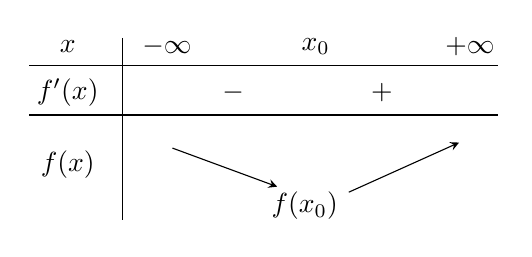
\begin{tikzpicture}[scale=0.7, >=stealth]
        % Các đường kẻ
        \draw (-1.5,0) -- (7,0);
        \draw (-1.5,-0.9) -- (7,-0.9);
        \draw (0.2,0.5) -- (0.2,-2.8);
        % Hàng x
        \node at (-0.8,0.35) {$x$};
        \node at (1,0.35) {$-\infty$};
        \node at (3.7,0.35) {$x_0$};
        \node at (6.5,0.35) {$+\infty$};
        % Hàng f'(x)
        \node at (-0.8,-0.5) {$f'(x)$};
        \node at (2.2,-0.5) {$-$};
        \node at (4.9,-0.5) {$+$};
        % Hàng f(x)
        \node at (-0.8,-1.8) {$f(x)$};
        % Mũi tên biến thiên
        \draw[->] (1.1,-1.5) -- (3.0,-2.2);
        \draw[->] (4.3,-2.3) -- (6.3,-1.4);
        % Giá trị cực tiểu
        \node at (3.5,-2.55) {$f(x_0)$};        
    \end{tikzpicture}  
    \hspace{1.5cm}
    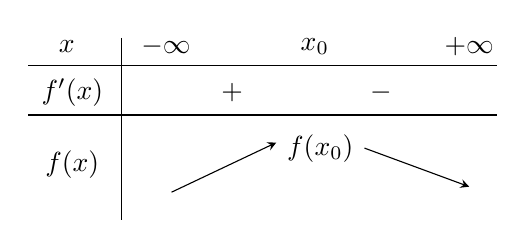
\begin{tikzpicture}[scale=0.7, >=stealth]        
        % Các đường kẻ
        \draw (8.5,0) -- (17,0);
        \draw (8.5,-0.9) -- (17,-0.9);
        \draw (10.2,0.5) -- (10.2,-2.8);        
        % Hàng x
        \node at (9.2,0.35) {$x$};
        \node at (11,0.35) {$-\infty$};
        \node at (13.7,0.35) {$x_0$};
        \node at (16.5,0.35) {$+\infty$};        
        % Hàng f'(x)
        \node at (9.3,-0.5) {$f'(x)$};
        \node at (12.2,-0.5) {$+$};
        \node at (14.9,-0.5) {$-$};        
        % Hàng f(x)
        \node at (9.3,-1.8) {$f(x)$};        
        % Mũi tên biến thiên
        \draw[->] (11.1,-2.3) -- (13.0,-1.4);
        \draw[->] (14.6,-1.5) -- (16.5,-2.2);        
        % Giá trị cực tiểu
        \node at (13.8,-1.5) {$f(x_0)$};       
    \end{tikzpicture}
    \subsection{Hàm đặc trưng}
        \begin{tc}
             Cho hàm số $y=f(x)$ đồng biến (hoặc nghịch biến) trên $K$. Khi đó với mọi $x \in K$:
             $$f(x_1)=f(x_2) \Leftrightarrow x_1=x_2; \quad f(x_1)>f(x_2) \Leftrightarrow x_1>x_2$$ 
        \end{tc}
        \begin{cy}
            Từ đó, trong nhiều bài toán, ta đưa phương trình về dạng $f(g(x)) = f(h(x))$ và biện luận nếu hàm $f(x)$ đơn điệu trên $K$ và $g(x), h(x)$ đều nhận giá trị trên $K$ thì phương trình $f(g(x)) = f(h(x)) \Leftrightarrow g(x) = h(x)$.
            \begin{itemize}
                \item[(i)] Nếu $f(x)$ đồng biến trên $K$ thì $f(g(x)) > f(h(x)) \Leftrightarrow g(x) > h(x)$.
                \item[(ii)] Nếu $f(x)$ nghịch biến trên $K$ thì $f(g(x)) < f(h(x)) \Leftrightarrow g(x) > h(x)$.
            \end{itemize}
        \end{cy}
        \begin{vd}
            Một phàn lát cắt của dãy núi có độ cao tính bằng mét được mô tả bởi hàm số
            $$y=h(x)=- \frac{1}{1320000}x^3+ \frac{9}{3520}x^2- \frac{81}{44}x+840 \text{ với } 0 \leq x \leq 2000$$
        \end{vd}
        \begin{center}
        
\includegraphics[width=0.9\textwidth]{Hinh2.png}
        \end{center}
        Tìm tọa độ các đỉnh của lát cắt dãy núi trên đoạn $[0;2000]$.
       
        Hướng dẫn giải:
        
        Ta có:
        $$h'(x)=- \frac{x^2}{440000}+ \frac{9x}{1760}- \frac{81}{44} \forall x \in (0;2000)$$

        Do đó $h'(x)=0 \Leftrightarrow 
            \left[
            \small \begin{aligned}
            x &= 450\\
            x &= 1800
            \end{aligned} 
            \right.
        $.
        Xét $h(450)=660,313$ và $h(1800)= \frac{15315}{11}$. 

        Do đó tọa độ các đỉnh của lát cắt dãy núi trên đoạn $[0;2000]$ là $(450;460,313)$ và $(1800; \dfrac{15315}{11})$.
    \section{Nền tảng về giá trị lớn nhất và giá trị nhỏ nhất của hàm số}
    \subsection{Định nghĩa}
        \begin{dn}
        Cho hàm số $f(x)$ xác định trên $D$.
        \end{dn}
        \begin{itemize}
            \item[(i)] Số $M$ được gọi là giá trị lớn nhất của hàm số $y=f(x)$ trên $D$, kí hiệu $M=max_Df(x)$ nếu
                \[
                \small \begin{cases}
                f(x) \leq M \forall x \in D\\
                \exists x_0 \in D| f(x_0)=M
                \end{cases}
                \]
            \item[(ii)] Số $m$ được gọi là giá trị nhỏ nhất của hàm số $y=f(x)$ trên $D$, kí hiệu $M=min_Df(x)$ nếu
                \[
                \small \begin{cases}
                f(x) \geq m \forall x \in D\\
                \exists x_0 \in D| f(x_0)=m
                \end{cases}
                \]
        \end{itemize}
    \subsection{Tìm giá trị lớn nhất và giá trị nhỏ nhất của hàm số liên tục}
        \begin{cy}
            Mọi hàm số liên tục trên một đoạn đều có giá trị lớn nhất và giá trị nhỏ nhất trên đoạn đó.
        \end{cy}
        Giả sử hàm số $f(x)$ liên tục trên đoạn $[a;b]$ và có đạo hàm trên khoảng $(a;b)$, có thể trừ đi một số hữu hạn điểm. Nếu $f'(x)=0$ chỉ tại một số hữu hạn điểm thuộc khoảng $(a;b)$ thì t có quy tắc tìm giá trị lớn nhất và giá trị nhỏ nhất của hàm số $f(x)$ trên đoạn $[a;b]$ như sau:
        \begin{itemize}
            \item[] \textit{Bước 1}. Tìm các điểm $x_1,x_2,...,x_n$ thuộc khoảng $(a;b)$ mà tại đó hàm số có đạo hàm bằng $0$ hoặc không tồn tại.
            \item[] \textit{Bước 2}. Tính $f(x_1),f(x_2),...,f(x_n),f(a) \text{ và } f(b)$.
            \item[] \textit{Bước 3}. So sánh các giá trị tìm được ở \textit{Bước 2}.
            \begin{nx}
                Số lớn nhất trong các giá trị đó là giá trị lớn nhát của hàm số $f(x)$ trên đoạn [a;b], số nhỏ nhát trong các giá trị đó là giá trị nhỏ nhất của hàm số $f(x)$ trên đoạn $[a;b]$.
            \end{nx}
        \end{itemize}
    \subsection{Lưu ý}
        \begin{itemize}
            \item[(i)] Lưu ý về giá trị lớn nhất và nhỏ nhất của hàm số $f(x)=asinx+bcosx$.\\
            Cho hàm số $f(x)=asinx+bcosx(a^2+b^2>0)$. Khi đó:
            $$maxf(x)= \sqrt{a^2+b^2};min f(x)=-\sqrt{a^2+b^2}$$
            \begin{hq}
                $max(asinx)= \lvert a \rvert; min(asinx)=-\lvert a \rvert$.
            \end{hq}
            \item[(ii)] Lưu ý về giá trị lớn nhất và giá trị nhỏ nhất của hàm số $f(u(x))$ trên $D$.\\
            Đặt $t=u(x)$, với $x \in D$, giả sử ta tìm được tập giá trị của $u(x)$ trên $D$ là $K$. Khi đó:
            $$max_{x\in D} f(u(x))= max_{i \in K} f(t)$$
            \item[(iii)] Bất đẳng thức Cauchy (BĐT AM-GM) cho 2 số và cho 3 số\\
            Cho $a,b$ là các số thực không âm, khi đó:
            $$\frac{a+b}{2} \geq \sqrt{ab}$$.
            Cho $a,b,c$ là các số thực không âm, khi đó:
            $$\frac{a+b+c}{3} \geq \sqrt[3]{abc}$$.
            \begin{hq}
                $ab \leq (\frac{a+b}{2})^2,abc \leq (\frac{a+b+c}{3})^3$ với $a,b,c \geq0$.
            \end{hq}
        \end{itemize}
        \begin{minipage}{0.68\textwidth}
        \begin{vd}
            Một miếng bìa hình tam giác đều $ABC$ có cạnh bằng $16$. Học sinh cắt một hình chữ nhật $MNPQ$ từ miếng bìa trên làm biển trông xe cho lớ học buổi ngoại khóa (với $M,N$ thuộc cạnh $BC$ và $P,Q$ lần lượt thuộc cạnh $AC$ và $AB$). Gọi $S$ là giá trị lớn nhất của diện tích hình chữ nhật $MNPQ$. Khi đó, giá trị $S^2$ bằng bao nhiêu?
        \end{vd}
        \end{minipage}
        \hfill
        \begin{minipage}{0.27\textwidth}
        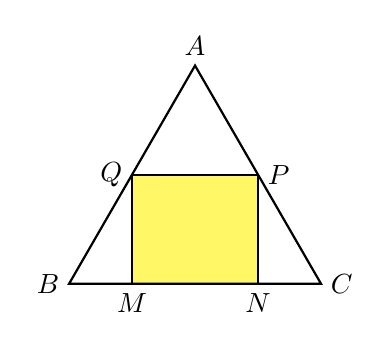
\begin{tikzpicture}[scale=0.4]
            % Các đỉnh tam giác
            \coordinate (A) at (4,6.928);
            \coordinate (B) at (0,0);
            \coordinate (C) at (8,0);
            % Các điểm
            \coordinate (M) at (2,0);
            \coordinate (N) at (6,0);
            \coordinate (Q) at (2,3.464);
            \coordinate (P) at (6,3.464);    
            % Tô hình chữ nhật
            \fill[yellow!60] (M) -- (N) -- (P) -- (Q) -- cycle;    
            % Tam giác
            \draw[thick] (A) -- (B) -- (C) -- cycle;
            % Hình chữ nhật
            \draw[thick] (M) -- (N) -- (P) -- (Q) -- cycle;
            % Nhãn
            \node[above] at (A) {$A$};
            \node[left] at (B) {$B$};
            \node[right] at (C) {$C$};
            \node[below] at (M) {$M$};
            \node[below] at (N) {$N$};
            \node[right] at (P) {$P$};
            \node[left] at (Q) {$Q$};
        \end{tikzpicture}
        \end{minipage}

        Hướng dẫn giải:
        
        Gọi $H$ là trung điểm của $BC$. Kẻ $AH$ cắt $PQ$ tại $K$.

         Đặt $PK=x$. Ta có $PQ=2x\;(0<x<8)$.
        \begin{center}
        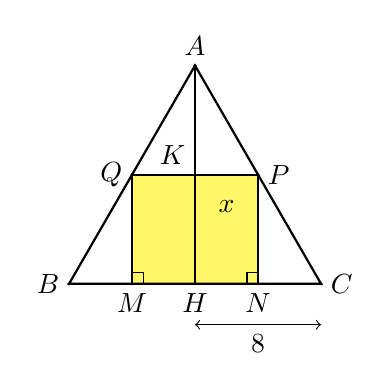
\begin{tikzpicture}[scale=0.4]
            % Các đỉnh tam giác
            \coordinate (A) at (4,6.928);
            \coordinate (B) at (0,0);
            \coordinate (C) at (8,0);
            % Các điểm
            \coordinate (M) at (2,0);
            \coordinate (N) at (6,0);
            \coordinate (H) at (4,0);
            \coordinate (Q) at (2,3.464);
            \coordinate (K) at (4,3.464);
            \coordinate (P) at (6,3.464);
            % Tô hình chữ nhật
            \fill[yellow!60] (M) -- (N) -- (P) -- (Q) -- cycle;
            % Tam giác ABC
            \draw[thick] (A) -- (B) -- (C) -- cycle;
            % Đường AH
            \draw[thick] (A) -- (H);
            % Hình chữ nhật MNPQ
            \draw[thick] (M) -- (N) -- (P) -- (Q) -- cycle;
            % Hai cạnh QM và PN
            \draw[thick] (Q) -- (M);
            \draw[thick] (P) -- (N);
            % Các điểm
            \fill (A) circle (1.5pt);
            \fill (B) circle (1.5pt);
            \fill (C) circle (1.5pt);
            \fill (M) circle (1.5pt);
            \fill (N) circle (1.5pt);
            \fill (H) circle (1.5pt);
            \fill (Q) circle (1.5pt);
            \fill (K) circle (1.5pt);
            \fill (P) circle (1.5pt);
            % Nhãn
            \node[above] at (A) {$A$};
            \node[left] at (B) {$B$};
            \node[right] at (C) {$C$};
            \node[below] at (M) {$M$};
            \node[below] at (N) {$N$};
            \node[below] at (H) {$H$};
            \node[left] at (Q) {$Q$};
            \node[above left] at (K) {$K$};
            \node[right] at (P) {$P$};
            % Đánh dấu x = KP
            \node at (5.0,2.45) {$x$};
            % Đánh dấu góc vuông tại M
            \draw (2,0.35) -- (2.35,0.35) -- (2.35,0);
            % Đánh dấu góc vuông tại N
            \draw (5.65,0) -- (5.65,0.35) -- (6,0.35);
            % Độ dài HC = 8
            \draw[<->] (4,-1.3) -- (8,-1.3);
            \node[below] at (6,-1.3) {$8$};
        \end{tikzpicture}
        \end{center}
        
        Có $PN \mathrel{/\!/} AH$ nên
        $
        \dfrac{PN}{AH}=\dfrac{CN}{CH}
        \Rightarrow \dfrac{PN}{\dfrac{\sqrt{3}}{2}BC}
        =\dfrac{8-x}{8} \Rightarrow  PN=\sqrt{3}(8-x).
        $
        
        Do đó $
        S_{MNPQ}
        =PQ.PN
        =2x\sqrt{3}(8-x)
        =2\sqrt{3}x(8-x)
        \leq
        2\sqrt{3}
        \left(\dfrac{x+8-x}{2}\right)^2.
        $
        
        (áp dụng $
        ab\leq\left(\dfrac{a+b}{2}\right)^2
        \forall a,b\in\mathbb{R}
        $).
        
        Vậy $S^2\leq(32\sqrt{3})^2=3072.$   
    \section{Tiệm cận của đồ thị hàm số}
    \subsection{Đường tiệm cận ngang}
        \begin{dn}
            Đường thẳng $y=y_0$ được gọi là \textit{đường tiệm cận ngang} của đồ thị hàm số $y=f(x)$ nếu:
            $$\lim_{x \to +\infty}f(x)=y_0 \text{ hoặc } \lim_{x \to -\infty}f(x)=y_0$$
        \end{dn}
        \begin{center}
        
\includegraphics[width=0.9\textwidth]{Hinh3.jpeg}
        \end{center}
    \subsection{Đường tiệm cận đứng}
        \begin{minipage}{0.63\textwidth}
        \begin{dn}
            Đường thẳng $x=x_0$ được gọi là \textit{đường tiệm cận đứng} của đồ thị hàm số $y=f(x)$ nếu ít nhất một trong các điều kiện sau được thỏa mãn:
             $$\lim_{x \to x_0^-}f(x)= +\infty;\quad lim_{x \to x_0^-}f(x)= -\infty;$$
             $$\lim_{x \to x_0^+}f(x)= +\infty;\quad lim_{x \to x_0^+}f(x)= -\infty.$$
        \end{dn}
        \end{minipage}
        \hfill
        \begin{minipage}{0.3\textwidth}
        
\includegraphics[width=0.9\textwidth]{Hinh4.png}
        \end{minipage}
    \subsection{Đường tiệm cận xiên}
        \begin{minipage}{0.63\textwidth}
        \begin{dn}
            Đường thẳng $y=ax+b(a \neq 0)$ được gọi là \textit{đường tiệm cận xiên} của đồ thị hàm số $y=f(x)$ nếu:
            $$\lim_{x \to +\infty}[f(x)-(ax+b)]=0 \text{ hoặc}
            \lim_{x \to -\infty}[f(x)-(ax+b)]=0$$
        \end{dn}
        \end{minipage}
        \hfill
        \begin{minipage}{0.3\textwidth}
        
\includegraphics[width=0.9\textwidth]{Hinh5.png}
        \end{minipage}
        \begin{nx}
            Để xác định hệ số $a,b,c$ của đường tiệm cận $y=ax+b$ của đồ thị hàm số $y=f(x)$, ta có thể áp dụng công thức sau:
            $$a=\lim_{x\to+\infty}\frac{f(x)}{x}\quad \text{và} \quad b=\lim_{x\to+\infty}\left[f(x)-ax\right].$$
            $$\text{hoặc} \quad a=\lim_{x\to+\infty}\frac{f(x)}{x} \quad\text{và}\quad b=\lim_{x\to+\infty}\left[f(x)-ax\right].$$
        \end{nx}
    \subsection{Một số lưu ý}
        \begin{ly}
            Một đồ thị hàm số có thể vừa có tiệm cận ngang, vừa có tiệm cận đứng, vừa có tiệm cận xiên.
        \end{ly}
        \begin{vd}
            Đồ thị hàm số $y= \sqrt{x^2+x+1}-x+ \frac{1}{x}$ có hình vẽ như sau:
        \end{vd}
        \begin{center}
        
\includegraphics[width=0.4\textwidth]{Hinh6.png}
        \end{center}
        Đồ thị hàm số này có đường tiệm cận xiên $y=-2x-\frac{1}{2}$, tiệm cận ngang $y=\frac{1}{2}$ và tiệm cận đứng $x=0$.
        \begin{ly}
            Đường tiệm cận ngang của đồ thị hàm số có thể cắt đồ thị tại vô số điểm
        \end{ly}
        \begin{ly}
             Đồ thị hàm số
$
y=\dfrac{\sin x}{x}
$
có
$
\displaystyle\lim_{x\to+\infty}y=0,
$
nên nhận đường $y=0$ làm tiệm cận xiên, và phương trình
$
\dfrac{\sin x}{x}=0
$
có vô số nghiệm.
        \end{ly}
        \begin{center}
        
\includegraphics[width=0.7\textwidth]{Hinh7.png}
        \end{center}
        \begin{ly}
            Để tìm tiệm cận xiên của đồ thị hàm số $y = \frac{ax^2 + bx + c}{mx + n} \quad (am \neq 0)$, ta làm như sau:

Phân tích $y = \dfrac{ax^2 + bx + c}{mx + n} = a'x + b' + \dfrac{c'}{mx + n}$ (có thể dùng phép chia đa thức), khi đó đường thẳng $y = a'x + b'$ là đường tiệm cận xiên của đồ thị hàm số đã cho.
\end{ly}
\begin{vd}
    Tìm tiệm cận xiên của đồ thị hàm số $y = \dfrac{10x^2 - 3x + 4}{5x + 6}$.
\end{vd}
\begin{center}
    \textbf{Giải}
\end{center}
Ta có: $y = 2x - 3 + \dfrac{22}{5x + 6}$. Do đó phương trình đường tiệm cận xiên: $y = 2x - 3$.
\begin{ly}
    Đồ thị hàm số $y = \ln x$ có đường tiệm cận đứng $x = 0$.

Khi tìm tiệm cận đứng của đồ thị hàm số $y = \ln u(x)$, ta nên giới hạn để $u(x) \to 0^+$.

\end{ly}
\begin{vd}
    Tìm các đường tiệm cận đứng của đồ thị hàm số $y = \ln(x^2 - 2x)$.
\end{vd}
\begin{center}
    \textbf{Giải}
\end{center}
Điều kiện: $x^2 - 2x > 0 \Leftrightarrow \left[ \begin{array}{l} x > 2 \\ x < 0 \end{array} \right.$. Dễ thấy $\displaystyle\lim_{x \to 2^+} y = -\infty$ và $\lim_{x \to 0^-} y = -\infty$ nên đồ thị hàm số có $2$ đường tiệm cận đứng là $x = 0$ và $x = 2$.
        \begin{center}
        
\includegraphics[width=0.4\textwidth]{Hinh8.png}
        \end{center}
        \begin{ly}
        Tiệm cận xiên của hàm căn thức

Xét hàm số $f(x) = \sqrt{ax^2 + bx + c} + px + q$ với $a > 0$. Tìm các đường tiệm cận của đồ thị hàm số.

\begin{itemize}
    \item Ta viết lại $f(x) = \sqrt{(\sqrt{a}x + m)^2 + n} + px + q$
    \item Đồ thị hàm số $y = f(x)$ có đường tiệm cận: $y = \pm(\sqrt{a}x + m) + px + q$.
\end{itemize}

\noindent \textbf{Chú ý:} Khi $a = p^2$, đồ thị hàm số có $1$ đường tiệm cận ngang và $1$ đường tiệm cận xiên.

\textbf{Một số ví dụ}
\begin{itemize}
    \item Đồ thị hàm số $y = \sqrt{x^2 + 1}$ có $2$ đường tiệm cận xiên là $y = x$ và $y = -x$.
\end{itemize}
        \end{ly}
        \begin{center}
        
\includegraphics[width=0.4\textwidth]{Hinh9.png}
        \end{center}
        \begin{itemize}
    \item Đồ thị hàm số $y = \sqrt{x^2-2x-5}$ có $2$ đường tiệm cận xiên là $y = x-1$ và $y = -x+1$.
\end{itemize}
        \begin{center}
        
\includegraphics[width=0.4\textwidth]{Hinh10.png}
        \end{center}\begin{itemize}
    \item Đồ thị hàm số $y = \sqrt{4x^2+4x+2}$ có đường tiệm cận xiên là $y = -4x-1$ và đường tiệm cận ngang là $y = 1$.
\end{itemize}
        \begin{center}
        
\includegraphics[width=0.4\textwidth]{Hinh11.png}
        \end{center}
    \section{Khảo sát đồ thị hàm số}
    \subsection{Đồ thị hàm số bậc hai}
        \begin{kn}
            \textbf{Hàm số bậc hai} là hàm số cho bởi công thức
$$y = ax^2 + bx + c$$
trong đó $x$ là biến số, $a$, $b$, $c$ là các hằng số và $a \neq 0$.

Tập xác định của hàm số bậc hai là $\mathbb{R}$.
        \end{kn}
        
        \textbf{\underline{Cách vẽ đồ thị hàm số bậc hai}}
        \begin{itemize}
    \item Đồ thị hàm số $y = ax^2 + bx + c$ ($a \neq 0$) là một đường parabol có đỉnh là điểm $I\left(-\frac{b}{2a}; -\frac{\Delta}{4a}\right)$, có trục đối xứng là đường thẳng $x = -\frac{b}{2a}$. Parabol này quay bề lõm lên trên nếu $a > 0$, xuống dưới nếu $a < 0$.
    
    \item Để vẽ đường parabol $y = ax^2 + bx + c$ ta tiến hành theo các bước sau:
    \begin{enumerate}
        \item Xác định toạ độ đỉnh $I\left(-\dfrac{b}{2a}; -\dfrac{\Delta}{4a}\right)$;
        \item Xác định trục đối xứng $x = -\dfrac{b}{2a}$;
        \item Xác định toạ độ các giao điểm của parabol với trục tung, trục hoành (nếu có) và một vài điểm đặc biệt trên parabol;
        \item Vẽ parabol.
    \end{enumerate}
\end{itemize}
\begin{center}
        
\includegraphics[width=0.7\textwidth]{Hinh12.png}
        
        Hình 6.11 (\textit{Sách giáo khoa Toán 10, tập 2})
        \end{center}
        \begin{nx}
Tổng quát, ta có thể viết hàm số bậc hai $y = ax^2 + bx + c$ ($a \neq 0$) dưới dạng
$$y = ax^2 + bx + c = a\left(x^2 + 2\dfrac{b}{2a}x + \dfrac{b^2}{4a^2}\right) - \dfrac{b^2}{4a} + c = a\left(x + \dfrac{b}{2a}\right)^2 - \dfrac{\Delta}{4a}, \text{ với } \Delta = b^2 - 4ac.$$

Ta thấy điểm $I\left(-\dfrac{b}{2a}; -\dfrac{\Delta}{4a}\right)$ thuộc đồ thị hàm số bậc hai và là một điểm đặc biệt, nó đóng vai trò như điểm $O(0; 0)$ của đồ thị hàm số $y = ax^2$. Cụ thể:
\begin{itemize}
    \item Nếu $a > 0$ thì $y = a\left(x + \dfrac{b}{2a}\right)^2 - \dfrac{\Delta}{4a} \geq -\dfrac{\Delta}{4a}$ với mọi $x$. Như vậy điểm $I$ là điểm thấp nhất trên đồ thị.
    \item Nếu $a < 0$ thì $y = a\left(x + \dfrac{b}{2a}\right)^2 - \dfrac{\Delta}{4a} \leq -\dfrac{\Delta}{4a}$ với mọi $x$. Như vậy điểm $I$ là điểm cao nhất trên đồ thị.
\end{itemize}

Gọi $(P_0)$ là parabol $y = ax^2$. Nếu ta ``dịch chuyển'' $(P_0)$ theo vectơ $\overrightarrow{OI}$ thì ta sẽ thu được đồ thị $(P)$ của hàm số $y = ax^2 + bx + c$ có dạng như Hình 6.11.
        \end{nx}
        \begin{nx}
         Từ đồ thị hàm số $y = ax^2 + bx + c$ ($a \neq 0$), ta suy ra tính chất của hàm số $y = ax^2 + bx + c$ ($a \neq 0$):

\vspace{0.3cm}

\begin{center}
\begin{tabular}{|p{7cm}|p{7cm}|}
    \hline
    \centering{Với $a > 0$} & \centering{Với $a < 0$} \tabularnewline % Hoặc Với a < 0
    \hline
    Hàm số nghịch biến trên khoảng $\left(-\infty; -\dfrac{b}{2a}\right)$;
    
    \vspace{0.2cm}
    Hàm số đồng biến trên khoảng $\left(-\dfrac{b}{2a}; +\infty\right)$;
    
    \vspace{0.2cm}
    $-\dfrac{\Delta}{4a}$ là giá trị nhỏ nhất của hàm số.
    & 
    Hàm số đồng biến trên khoảng $\left(-\infty; -\dfrac{b}{2a}\right)$;
    
    \vspace{0.2cm}
    Hàm số nghịch biến trên khoảng $\left(-\dfrac{b}{2a}; +\infty\right)$;
    
    \vspace{0.2cm}
    $-\dfrac{\Delta}{4a}$ là giá trị lớn nhất của hàm số.
    \vspace{0.2cm}
    \tabularnewline
    \hline
\end{tabular}
\end{center}
        \end{nx}
    \subsection{Đồ thị hàm số bậc ba}
    Cho hàm số $f(x)=ax^3+bx^2+cx+d (a\neq0),f'(x)=3ax^2+2bx+c,\Delta'=b^2-3ac$
\begin{center}
\begin{tabular}{|c|c|c|c|}
\hline
    & $\Delta' < 0$ & $\Delta' = 0$ & $\Delta' > 0$ \tabularnewline
    \hline
    \textbf{$a > 0$} & 
    % Ô 1: a > 0, delta' < 0 (Chèn hình ảnh đồ thị hoặc phác họa nếu cần)
    \begin{tabular}{c}
        
\includegraphics[width=0.1\textwidth]{Hinh13.png}
    \end{tabular} & 
    % Ô 2: a > 0, delta' = 0
    \begin{tabular}{c}
        
\includegraphics[width=0.1\textwidth]{Hinh14.png}
    \end{tabular} & 
    % Ô 3: a > 0, delta' > 0
    \begin{tabular}{c}
        
\includegraphics[width=0.15\textwidth]{Hinh15.png}
    \end{tabular} 
    \tabularnewline
    \hline
    \textbf{$a < 0$} & 
    % Ô 4: a < 0, delta' < 0
    \begin{tabular}{c}
        
\includegraphics[width=0.1\textwidth]{Hinh16.png}
    \end{tabular} & 
    % Ô 5: a < 0, delta' = 0
    \begin{tabular}{c}
        
\includegraphics[width=0.1\textwidth]{Hinh17.png}
    \end{tabular} & 
    % Ô 6: a < 0, delta' > 0
    \begin{tabular}{c}
        
\includegraphics[width=0.15\textwidth]{Hinh18.png}
    \end{tabular} 
    \tabularnewline
    \hline
\end{tabular}
\end{center}
Điểm uốn của đồ thị hàm số bậc ba là tâm đối xứng của đồ thị.

Xét $f''(x) = 6ax + 2b$; $f''(x) = 0 \iff x = \dfrac{-b}{3a}$.

Điểm $U\left(-\dfrac{b}{3a}; f\left(-\dfrac{b}{3a}\right)\right)$ là điểm uốn của đồ thị.

Đồ thị hàm số bậc ba có thể không có cực trị, hoặc có thể có đúng 2 điểm cực trị.
    \subsection{Đồ thị hàm số bậc nhất trên bậc nhất}
    Xét hàm số $f(x)=\dfrac{ax+b}{cx+d} (c\neq0)$.
    
\begin{center}
\begin{tabular}{|c|c|}
    \hline
    \textbf{$ad - bc < 0$} & \textbf{$ad - bc > 0$} \tabularnewline
    \hline
    % Ô 1: ad - bc < 0 (Hàm số nghịch biến trên các khoảng xác định)
    \begin{tabular}{c}
        
\includegraphics[width=0.3\textwidth]{Hinh19.png}
    \end{tabular} & 
    % Ô 2: ad - bc > 0 (Hàm số đồng biến trên các khoảng xác định)
    \begin{tabular}{c}
        
\includegraphics[width=0.35\textwidth]{Hinh20.png}
    \end{tabular} 
    \tabularnewline
    \hline
\end{tabular}
\end{center}
        \begin{nx}
Đồ thị hàm số có 2 đường tiệm cận:
\begin{itemize}
    \item Tiệm cận ngang: $y = \dfrac{a}{c}$
    \item Tiệm cận đứng: $x = -\dfrac{d}{c}$
\end{itemize}
Giao điểm hai đường tiệm cận là tâm đối xứng của đồ thị hàm số, hay tâm đối xứng $I$ có tọa độ là $I\left(-\dfrac{d}{c}; \dfrac{a}{c}\right)$.

Hàm số $f(x)$ luôn đồng biến (hoặc nghịch biến) trên các khoảng xác định.
        \end{nx}
    \subsection{Đồ thị hàm số bậc hai trên bậc nhất}
    Xét hàm số $f(x)=\dfrac{ax^2+bx+c}{px+q} \text{ với }a \neq0, p \neq0,$ đa thức tử không chia hết cho đa thức mẫu.
\begin{center}
\begin{tabular}{|c|c|}
    \hline
    % Ô hàng 1, cột 1
    \begin{tabular}{c}
        
\includegraphics[width=0.35\textwidth]{Hinh21.png}
    \end{tabular} & 
    % Ô hàng 1, cột 2
    \begin{tabular}{c}
        
\includegraphics[width=0.33\textwidth]{Hinh22.png}
    \end{tabular} 
    \tabularnewline
    \hline
    % Ô hàng 2, cột 1
    \begin{tabular}{c}
        
\includegraphics[width=0.35\textwidth]{Hinh23.png}
    \end{tabular} & 
    % Ô hàng 2, cột 2
    \begin{tabular}{c}
       
\includegraphics[width=0.33\textwidth]{Hinh24.png}
    \end{tabular} 
    \tabularnewline
    \hline
\end{tabular}
\end{center}
\begin{nx}
Đồ thị hàm số có 2 đường tiệm cận:
\begin{itemize}
    \item \textbf{Tiệm cận xiên:} Viết lại $f(x) = mx + n + \frac{k}{px + q}$ ($m \neq 0$) thì đồ thị hàm số nhận đường $y = mx + n$ làm đường tiệm cận xiên.
    \item \textbf{Tiệm cận đứng:} $x = -\frac{q}{p}$.
    \item Đồ thị hàm số nhận giao điểm của hai đường tiệm cận làm tâm đối xứng.
    \item Đồ thị hàm số nhận đường phân giác của các góc tạo bởi hai đường tiệm cận này làm các trục đối xứng.
\end{itemize}
\end{nx}
%%%%%%%%%%%%%%%%%%%%%%%%%%%%%%%%%%%%%%%%%%%%%%%%
    \chapter{MỘT SỐ BÀI TOÁN THỰC TẾ ỨNG DỤNG ĐỒ THỊ HÀM SỐ}
    Dựa trên nền tảng lý thuyết và quy trình khảo sát hàm số đã trình bày ở Chương 1, Chương 2 tập trung xây dựng, phân tích và giải quyết một hệ thống các bài toán thực tế đa dạng. Thông qua việc phân tích lời giải chi tiết, đưa ra các nhận xét, ý tưởng, lưu ý tính toán và đánh giá dưới góc độ sư phạm, chương này làm rõ vai trò của đồ thị hàm số như một công cụ hiệu quả trong việc mô hình hóa toán học các tình huống thực tiễn.
    \section{Đồ thị hàm số đa thức trong các bài toán thực tế}
    \subsection{Đồ thị hàm số bậc hai}
%%%%%%%%%%%%%%%%%%%%%%%%%%%%%%%%%%%%%%%%%%%%%%%%%%%%%%%%%%%%%%%%%%%%%%%%%%%%%%%%%%%%
        \textbf{\underline{Bài toán $1$:}}

        Người ta muốn làm sàn nổi nối liền trên một sân khấu nổi trên mặt hồ có tiết diện là phần hình chữ nhật $ABDC$, nằm ở phần trong giới hạn bởi đồ thị hàm số $y = x^2 - 2x - 2$ và đồ thị hàm số $y = -\dfrac{1}{2}x^2 + x + \dfrac{5}{2}$ ($AB$ song song với trục hoành, mỗi đơn vị trên hệ trục tọa độ dài $10\text{ m}$). Để làm sàn nổi, người ta phải bỏ ra $50.000\text{ VNĐ/m}^2$. Tính số tiền lớn nhất (đơn vị triệu đồng) mà người ta phải bỏ ra khi làm sàn nổi (kết quả làm tròn đến hàng phần chục).
        \begin{center}
            
\includegraphics[width=0.3\textwidth]{Hinh25.png}
        \end{center}
        
        \textbf{\underline{Nhận xét:}}
         Bài toán được lựa chọn vì có bối cảnh thực tế rõ ràng, trong đó hình dạng của sàn nổi được mô hình hóa bằng đồ thị của hai hàm số bậc hai. Việc xác định diện tích lớn nhất của hình chữ nhật $ABCD$ tạo ra mối liên hệ trực tiếp giữa đồ thị hàm số bậc hai và bài toán tối ưu trong thực tế. Qua bài toán, các đặc điểm của đồ thị như giao điểm, tính đối xứng và sự biến thiên có thể được khai thác để giải quyết vấn đề về diện tích và chi phí.
         
         \textbf{\underline{Ý tưởng giải:}}
         Đưa bài toán về bài toán tìm giá trị lớn nhất của diện tích hình chữ nhật $ABCD$. Dựa vào giao điểm của các đường thẳng song song với trục hoành và hai đồ thị parabol, biểu diễn chiều dài, chiều rộng của hình chữ nhật theo một biến; từ đó lập hàm diện tích và tìm giá trị lớn nhất.

         \textbf{\underline{Hướng dẫn giải:}}

         Bước 1. Xác định toạ độ các điểm
\begin{itemize}
    \item Dựa theo hình vẽ ta thấy $A$ và $B$ nằm trên đồ thị hàm số $y = -\dfrac{1}{2}x^2 + x + \dfrac{5}{2}$, $C$ và $D$ nằm trên đồ thị hàm số $y = x^2 - 2x - 2$.
    \item Hai parabol cắt nhau tại 2 điểm có hoành độ lần lượt là $x = -1$ và $x = 3$.
    \item Hai parabol có đỉnh nằm trên đường thẳng $x = 1$. Dựa theo tính chất đối xứng thì $x_A + x_B = 2$.
    \item Gọi $A\left(a; -\dfrac{1}{2}a^2 + a + \dfrac{5}{2}\right)$ ($-1 \le a \le 1$). Vì $AB \parallel Ox$ nên $B\left(2 - a; -\dfrac{1}{2}a^2 + a + \dfrac{5}{2}\right)$.
    \item Vì $ABDC$ là hình chữ nhật, $AB \parallel Ox \Rightarrow AC \parallel Oy \Rightarrow x_C = x_A = a$. Lại có $C$ thuộc đồ thị hàm số $y = x^2 - 2x - 2 \Rightarrow C(a; a^2 - 2a - 2)$.
\end{itemize}

Bước 2. Tính độ dài các cạnh
\begin{itemize}
    \item $AB \parallel Ox$ nên $AB = |x_B - x_A| = x_B - x_A = 2 - a - a = 2 - 2a$.
    \item $AC \parallel Oy$ nên $AC = |y_A - y_C| = y_A - y_C = -\dfrac{1}{2}a^2 + a + \dfrac{5}{2} - a^2 + 2a + 2 = -\dfrac{3}{2}a^2 + 3a + \dfrac{9}{2}$.
\end{itemize}

Bước 3. Tối ưu
\begin{itemize}
    \item Diện tích sàn nổi chính là diện tích hình chữ nhật $ABDC$ và bằng:
    $$S(a) = S_{ABDC} = AB \cdot AC = (2 - 2a)\left(-\dfrac{3}{2}a^2 + 3a + \frac{9}{2}\right) = (a - 1)(3a^2 - 6a - 9)$$
    \item Ta có: $S'(a) = 3a^2 - 6a - 9 + (a - 1)(6a - 6) = 9a^2 - 18a - 3$.
    \item Hàm số $S(a)$ liên tục trên $[-1; 1]$ có $S'(a) = 0 \iff a_0 = \dfrac{3 - 2\sqrt{3}}{3}$ nên:
    $$\max_{[-1; 1]} S(a) = \max\{S(-1); S(a_0); S(1)\} = S(a_0) = \dfrac{16\sqrt{3}}{3}$$
    \item Suy ra diện tích sàn nổi lớn nhất bằng $\dfrac{16\sqrt{3}}{3} \times 10^2 = \dfrac{1600\sqrt{3}}{3}\text{ m}^2$.
    \item Vậy số tiền lớn nhất phải bỏ ra bằng $\dfrac{1600\sqrt{3}}{3} \times 0,05 = \dfrac{80\sqrt{3}}{3} \approx 46,2\text{ triệu đồng}$.
\end{itemize}
        \textbf{\underline{Những lưu ý khi giải bài toán:}}
        Cần xác định chính xác đơn vị thực tế tương ứng với đơn vị trên hệ trục tọa độ trước khi tính diện tích.

Cần dựa vào điều kiện $AB \parallel Ox, CD \parallel Ox$ để xác định các giao điểm của hình chữ nhật với hai parabol.

Sau khi lập được hàm diện tích, phải xác định đúng miền giá trị của biến trước khi tìm giá trị lớn nhất.

Cuối cùng cần đổi đơn vị và tính chi phí theo dữ kiện $50.000\text{ đồng/m}^2$, đồng thời làm tròn theo yêu cầu đề bài.

        \textbf{\underline{Kết luận sư phạm:}}

        Bài toán có tính thực tế và thể hiện khá rõ khả năng ứng dụng đồ thị hàm số bậc hai vào một bài toán tối ưu trong thực tiễn. Việc chuyển từ hình dạng của sàn nổi được mô tả bởi hai parabol sang bài toán tìm diện tích lớn nhất giúp làm nổi bật vai trò của đồ thị hàm số trong việc mô hình hóa các tình huống thực tế.
        
        \textbf{Ưu điểm:}
        \begin{itemize}
            \item Bối cảnh thực tế cụ thể, dễ hình dung: thiết kế sàn nổi và tính chi phí.
            \item Có sự liên hệ trực tiếp giữa đồ thị hai hàm số bậc hai và bài toán tìm diện tích lớn nhất.
            \item Kết hợp được kiến thức đại số, hình học và đồ thị, tạo nên một bài toán có nhiều bước suy luận.
            \item Kết quả cuối cùng có ý nghĩa thực tế, chuyển từ diện tích sang chi phí.
        \end{itemize}
        
        \textbf{Nhược điểm:}
        \begin{itemize}
            \item Dữ kiện và hình vẽ chưa thật sự rõ ràng, đặc biệt là tỉ lệ của hai trục tọa độ.
            \item Học sinh có thể gặp khó khăn trong việc xác định tọa độ các đỉnh $A,B,C,D$ và thiết lập biểu thức diện tích.
            \item Bối cảnh thực tế còn mang tính giả định khá nhiều; mối quan hệ giữa hai parabol và hình dạng thực tế của sàn chưa được giải thích rõ.
        \end{itemize}
%%%%%%%%%%%%%%%%%%%%%%%%%%%%%%%%%%%%%%%%%%%%%%%%%%%%%%%%%%%%%%%%%%%%%%%%%%%%%%%%%%%%%        
        \textbf{\underline{Bài toán $2$:}}

        Một tuyến cáp treo trên núi chạy từ ga dưới của thung lũng đến một cột trụ trung gian, đoạn này có độ dài $1000\text{ m}$ theo phương ngang. Đoạn thứ hai nối tiếp từ cột trụ lên đến ga nằm trên đỉnh núi và có chiều dài là $3\text{ km}$.

Hình vẽ biểu diễn sơ đồ đường đi của cáp treo cũng như mặt cắt ngang bên dưới của ngọn núi. Trong hệ tọa độ được sử dụng, trục $Ox$ biểu thị khoảng cách theo phương ngang từ ga dưới và trục $Oy$ biểu thị độ cao so với mực nước biển. Mỗi đơn vị trên hệ trục tọa độ dài $1\text{ km}$ trong thực tế.

Trong đoạn dưới, đường đi của cáp treo được mô tả bởi hàm số
$$f(x) = 0,34x^2 + 0,15x + 1,16, \forall x \in [0; 1].$$

Trong đoạn trên, đường đi của cáp treo được mô tả bởi hàm số
$$g(x) = ax^2 + bx + c, \forall x \in [1; 4] \text{ với } a, b, c \in \mathbb{R}.$$

Độ dốc lớn nhất của đường đi cáp treo ở đoạn trên là $1,1$. Cáp treo ở ga trên có độ cao $3150\text{ m}$ so với mực nước biển. Độ cao của ngọn núi được mô hình hóa cho khu vực $1 \le x \le 3$ bằng hàm số $h(x) = 0,1x + 1,43$. Đối với độ cao này, tính khoảng cách theo phương thẳng đứng nhỏ nhất giữa cáp treo và ngọn núi (đơn vị mét).
        \begin{center}
            
\includegraphics[width=0.4\textwidth]{Hinh26.png}
        \end{center}
        
        \textbf{\underline{Nhận xét:}}
         
         Bài toán có sự gắn kết rõ ràng giữa đồ thị hàm số bậc hai và một tình huống thực tế về đường đi của cáp treo trên núi. Đường đi của cáp được mô hình hóa bằng các hàm số, trong đó đoạn trên được biểu diễn bởi một hàm số bậc hai chưa xác định. Các dữ kiện về độ dốc và độ cao được sử dụng để xác định hàm số, sau đó vận dụng hàm số để giải quyết vấn đề khoảng cách trong thực tế. Vì vậy, bài toán được lựa chọn nhằm minh họa cho việc sử dụng hàm số bậc hai để mô hình hóa và giải quyết các vấn đề liên quan đến địa hình, giao thông và xây dựng.
         
         \textbf{\underline{Ý tưởng giải:}}

        Trước hết, sử dụng các dữ kiện về độ cao của cáp tại \(x=1\), \(x=4\) và độ dốc lớn nhất để xác định các hệ số \(a,b,c\) của hàm số bậc hai \(g(x)\). Sau đó, so sánh \(g(x)\) với hàm số \(h(x)\) biểu diễn độ cao của ngọn núi để thiết lập khoảng cách theo phương thẳng đứng giữa cáp treo và ngọn núi. Cuối cùng, tìm giá trị nhỏ nhất của khoảng cách này trên đoạn xét.
        
         \textbf{\underline{Hướng dẫn giải:}}
            
            Bước 1. Phân tích dữ kiện
\begin{itemize}
    \item Trục $Ox$: khoảng cách ngang; trục $Oy$: độ cao so với mực nước biển (đơn vị: $\text{km}$).
    \item Đường đi trong đoạn dưới: $f(x) = 0,34x^2 + 0,15x + 1,16; \forall x \in [0; 1]$.
    \item Đường đi trong đoạn trên: $g(x) = ax^2 + bx + c, \forall x \in [1; 4]$.
    \item Độ dốc lớn nhất trong đoạn trên: $\max_{[1; 4]} g'(x) = 1,1$.
    \item Độ cao ở ga trên: $g(4) = 3,15 \text{ km}$.
    \item Độ cao núi (ở khu vực $1 \le x \le 3$) là $h(x) = 0,1x + 1,43$.
\end{itemize}

Bước 2. Xác định $g(x)$
\begin{itemize}
    \item Liên tục tại cột trung gian nên $g(1) = f(1) = 1,65$.
    \item $g'(x) = 2ax + b$ đồng biến trên $[1; 4] \Rightarrow \max_{[1; 4]} g'(x) = g'(4) = 1,1$. Khi đó:
    $$\begin{cases} g(1) = 1,65 \\ g(4) = 3,15 \\ g'(4) = 1,1 \end{cases} \Leftrightarrow \begin{cases} a + b + c = 1,65 \\ 16a + 4b + c = 3,15 \\ 8a + b = 1,1 \end{cases} \Leftrightarrow \begin{cases} a = 0,2 \\ b = -0,5 \\ c = 1,95 \end{cases}$$\\
    $\Rightarrow g(x) = 0,2x^2 - 0,5x + 1,95.$
\end{itemize}

Bước 3. Khoảng cách theo phương thẳng đứng và tối ưu
\begin{itemize}
    \item Trong khu vực $1 \le x \le 3$, khoảng cách theo phương thẳng đứng giữa cáp treo và ngọn núi bằng
    $$d(x) = (0,2x^2 - 0,5x + 1,95) - (0,1x + 1,43) = 0,2x^2 - 0,6x + 0,52$$
    \item Hàm số $d(x)$ là hàm số bậc hai có $a = 0,2 > 0$ nên nhận giá trị nhỏ nhất tại
    $$x_0 = -\dfrac{b}{2a} = \dfrac{-0,6}{2 \cdot 0,2} = \dfrac{3}{2}$$
    \item Vậy khoảng cách theo phương thẳng đứng nhỏ nhất giữa cáp treo và ngọn núi là $d(x_0) = 0,07 \text{ (km)} = 70 \text{ (m)}$
\end{itemize}
         
        \textbf{\underline{Những lưu ý khi giải bài toán:}}

        Khi giải cần chú ý đúng đơn vị của các đại lượng, xác định chính xác miền xét của từng hàm số và diễn giải “độ dốc lớn nhất” phù hợp với tính chất của hàm số bậc hai. Đặc biệt, khi tính khoảng cách giữa cáp và núi cần xác định đúng khoảng giá trị của \(x\) mà cả hai hàm số cùng biểu diễn các đối tượng thực tế.
        
        \textbf{\underline{Kết luận sư phạm:}}

       Bài toán là một ví dụ tiêu biểu cho việc ứng dụng hàm số bậc hai vào mô hình hóa các tình huống thực tế, trong đó đồ thị hàm số không chỉ được sử dụng để biểu diễn một đại lượng mà còn là cơ sở để giải quyết vấn đề về khoảng cách trong thực tế.
        
        \textbf{Ưu điểm:}
        \begin{itemize}
            \item Bối cảnh thực tế cụ thể, dễ hình dung.
            \item Thể hiện rõ mối liên hệ giữa hàm số bậc hai và đồ thị với vấn đề thực tế.
            \item Khai thác được nhiều đặc trưng của hàm số bậc hai như giá trị hàm số, độ dốc và sự biến thiên.
            \item Có quá trình chuyển từ dữ kiện thực tế → mô hình hàm số → kết quả thực tế.
        \end{itemize}
        
        \textbf{Nhược điểm:}
        \begin{itemize}
            \item Bài toán có nhiều dữ kiện và gồm nhiều bước xử lý liên tiếp.
            \item Khái niệm “độ dốc lớn nhất” cần được diễn giải rõ để chuyển thành điều kiện toán học.
            \item Hình vẽ và hệ tọa độ mang tính mô hình hóa, chưa phản ánh đầy đủ các yếu tố của địa hình thực tế.
        \end{itemize}
%%%%%%%%%%%%%%%%%%%%%%%%%%%%%%%%%%%%%%%%%%%%%%%%%%%%%%%%%%%%%%%%%%%%%%%%%%%%%%%%%%%%%
    \subsection{Đồ thị hàm số bậc ba}
     \textbf{\underline{Bài toán $3$:}}
        Khuôn viên của một công viên có dạng hình chữ nhật $ABCD$ với $AB = 100\text{ m}$; $AD = 80\text{ m}$. Người ta muốn chia công viên thành hai khu gồm một khu dành cho trẻ em, một khu dành cho người lớn. Để tạo thiết kế độc đáo và lạ mắt, người ta dùng một đường cong chia khuôn viên thành hai phần $H_1$ (không tô màu) dành cho người lớn và $H_2$ (tô màu) dành cho trẻ em như hình vẽ bên với $AH = 40\text{ m}$; $AE = 50\text{ m}$; $AP = 20\text{ m}$ và $EF \parallel AB$; $PQ \parallel AD$. Biết rằng khi xét trong hệ tọa độ $Oxy$, đường cong trong hình là một phần của một hàm số bậc ba. Phần chính giữa của công viên người ta muốn mắc dây đèn trang trí dọc theo đoạn thẳng $MN$ như hình. Biết giá tiền mỗi mét dây trang trí của phần dành cho trẻ em là $120$ nghìn đồng và phần dành cho người lớn là $200$ nghìn đồng. Tổng số tiền mắc dây đèn trang trí trên đoạn $MN$ là bao nhiêu triệu đồng?
       
        \begin{center}
            
\includegraphics[width=0.35\textwidth]{Hinh27.png}
        \end{center}
        
        \textbf{\underline{Nhận xét:}}
         
         Bài toán được lựa chọn vì có sự gắn kết giữa đồ thị hàm số bậc ba và một tình huống thực tế về thiết kế, phân chia không gian trong công viên. Đường cong chia công viên thành hai khu được mô hình hóa bằng một phần đồ thị hàm số bậc ba. Từ đó, các đặc điểm của đồ thị được sử dụng để xác định vị trí đường cong và tính độ dài các đoạn dây đèn thuộc hai khu vực, qua đó tính chi phí trang trí.
         
         \textbf{\underline{Ý tưởng giải:}}

         Dựa vào các dữ kiện hình học và các điểm thuộc đường cong để xác định hàm số bậc ba biểu diễn đường cong. Sau đó, xác định giao điểm của đường cong với đoạn \(MN\), từ đó tính độ dài phần \(MN\) thuộc khu dành cho trẻ em và phần thuộc khu dành cho người lớn. Cuối cùng, tính tổng chi phí dựa trên đơn giá của từng khu vực.
         
         \textbf{\underline{Hướng dẫn giải:}}
                
                Bước 1. Đặt hệ trục và toạ độ
\begin{itemize}
    \item Chọn $A$ trùng với gốc toạ độ $O$; trục $Ox$ trùng với $AB$, trục $Oy$ trùng với $AD$; mỗi đơn vị trên hệ trục toạ độ ứng với $10\text{ m}$.
    \item Khi đó $H(0; 4)$; $E(0; 5)$; $P(2; 0)$; $B(10; 0)$; $D(0; 8)$. Vì $EF \parallel AB$; $PQ \parallel AD$ nên suy ra $Q(2; 5)$; $F(10; 5)$.
\end{itemize}

Bước 2. Xác định phương trình đường cong
\begin{itemize}
    \item Đường cong trong hình là một phần của đồ thị hàm số bậc ba có dạng
    $$y = f(x) = ax^3 + bx^2 + cx + d$$
    \item Suy ra $f'(x) = 3ax^2 + 2bx + c$
    \item Đường cong $f(x)$ đi qua điểm $H$; điểm $F$ có $Q$ là điểm cực trị nên
    $$\begin{cases} f(0) = 4 \\ f(2) = 5 \\ f(10) = 5 \\ f'(2) = 0 \end{cases} \Leftrightarrow \begin{cases} d = 4 \\ 8a + 4b + 2c + d = 5 \\ 1000a + 100b + 10c + d = 5 \\ 12a + 4b + c = 0 \end{cases} \Leftrightarrow \begin{cases} a = \dfrac{1}{40} \\ b = -\dfrac{7}{20} \\ c = \dfrac{11}{10} \\ d = 4 \end{cases}$$
    $$\Rightarrow f(x) = \dfrac{1}{40}x^3 - \dfrac{7}{20}x^2 + \dfrac{11}{10}x + 4$$
\end{itemize}

Bước 3. Tính tổng số tiền
\begin{itemize}
    \item Khi đó độ dài đoạn thẳng $IM = f(5) \times 10 = 38,75\text{ m}$.
    \item Độ dài đoạn thẳng $IN$ bằng $MN - IM = 80 - 38,75 = 41,25\text{ m}$.
    \item Tổng số tiền bao gồm số tiền dây trang trí của phần trẻ em là đoạn thẳng $IM$ và số tiền dây trang trí của phần người lớn là đoạn thẳng $IN$.
\end{itemize}

Tổng số tiền là: $120 \cdot 38,75 + 200 \cdot 41,25 = 12\,900\text{ (nghìn đồng)} {= 12,9}\text{ triệu đồng}$.
         
        \textbf{\underline{Những lưu ý khi giải bài toán:}}
        \begin{itemize}
            \item Cần xác định chính xác hệ tọa độ và tọa độ các điểm dựa trên hình vẽ.
            \item Sử dụng đầy đủ các dữ kiện để xác định hàm số bậc ba, tránh chỉ dựa vào hình dạng trực quan của đường cong.
            \item Xác định chính xác giao điểm của đường cong với \(MN\) để phân chia độ dài dây đèn theo từng khu.
            \item Cần chú ý đơn vị mét và đổi sang triệu đồng ở bước tính chi phí.
        \end{itemize}
        
        \textbf{\underline{Kết luận sư phạm:}}

        Bài toán là một ví dụ về ứng dụng đồ thị hàm số bậc ba trong mô hình hóa một tình huống thực tế, trong đó đồ thị được sử dụng để mô tả một đường cong có hình dạng phức tạp hơn đường thẳng hoặc parabol. Bài toán đồng thời tạo ra sự kết nối giữa kiến thức về hàm số bậc ba với các vấn đề thực tế như thiết kế không gian và tính toán chi phí.       
        
        \textbf{Ưu điểm:}
        \begin{itemize}
            \item Bối cảnh thực tế gần gũi, gắn với thiết kế công viên.
            \item Thể hiện rõ vai trò của đồ thị hàm số bậc ba trong mô hình hóa đường cong.
            \item Kết hợp kiến thức hàm số với kiến thức hình học và bài toán chi phí.
            \item Kết quả cuối cùng có ý nghĩa thực tế, dễ liên hệ với tình huống ban đầu.
        \end{itemize}
        
        \textbf{Nhược điểm:}
        \begin{itemize}
            \item Bài toán có nhiều dữ kiện hình học, có thể gây khó khăn khi chuyển từ hình vẽ sang mô hình hàm số.
            \item Việc xác định hàm số bậc ba đòi hỏi xử lý nhiều điều kiện.
            \item Phần tính toán độ dài \(MN\) phụ thuộc khá nhiều vào việc đọc chính xác hình vẽ và xác định vị trí giao điểm.
        \end{itemize}
%%%%%%%%%%%%%%%%%%%%%%%%%%%%%%%%%%%%%%%%%%%%%%%%%%%%%%%%%%%%%%%%%%%%%%%%%%%%%%%%%%%%%
    
    \textbf{\underline{Bài toán $4$:}}

        Một hồ nước nhân tạo được xây dựng trong một công viên giải trí. Trong mô hình minh hoạ, nó được giới hạn bởi các trục toạ độ và đồ thị hàm số $y = f(x) = \frac{1}{10}(-x^3 + 9x^2 - 15x + 56)$. Đơn vị đo độ dài trên mỗi trục toạ độ là $100\text{ m}$.

\begin{enumerate}[a)]
    \item Đường dạo ven hồ chạy dọc theo trục $Ox$ dài $600\text{ m}$.
    \item Trên đường đi dạo ven hồ chạy dọc theo trục $Ox$, điểm cách gốc $O$ một đoạn $500\text{ m}$ có khoảng cách theo phương thẳng đứng đến bờ hồ đối diện là lớn nhất.
    \item Xét trong $500$ mét đầu tiên theo phương nằm ngang của đường đi dạo ven hồ, khoảng cách nhỏ nhất theo phương thẳng đứng từ một điểm trên đường đi dạo ven hồ dọc theo trục $Ox$ đến bờ hồ đối diện là $490\text{ m}$.
    \item Trong công viên có một con đường chạy dọc theo đồ thị hàm số $y = -1,5x + 18$. Người ta dự định xây dựng bên bờ hồ một bến thuyền đạp nước sao cho khoảng cách từ bến thuyền đến con đường này là ngắn nhất. Biết toạ độ của điểm để xây bến thuyền này là $M(a; b)$. Giá trị $a + 5b$ bằng $43$.
\end{enumerate}

        Xác định tính đúng sai của các mệnh đề trên.
        \begin{center}
            
\includegraphics[width=0.4\textwidth]{Hinh28.png}
        \end{center}
        
        \textbf{\underline{Nhận xét:}}

        Bài toán được lựa chọn vì có sự kết nối trực tiếp giữa đồ thị hàm số bậc ba và một tình huống thực tế về thiết kế hồ nước, đường dạo và bến thuyền trong công viên. Đồ thị hàm số được sử dụng để mô hình hóa bờ hồ, từ đó khai thác các đặc điểm của đồ thị để giải quyết những vấn đề về khoảng cách, vị trí và thiết kế trong thực tế. Đặc biệt, bài toán cho thấy đồ thị hàm số bậc ba có thể được sử dụng để mô tả những đường cong có hình dạng phức tạp trong các mô hình thực tế.
         
         \textbf{\underline{Ý tưởng giải:}}

         Dựa vào hàm số đã cho và tỉ lệ của hệ trục tọa độ để xác định các đại lượng thực tế. Với các mệnh đề về khoảng cách theo phương thẳng đứng, xét giá trị của hàm số trên các khoảng tương ứng để xác định giá trị lớn nhất, nhỏ nhất. Với mệnh đề về bến thuyền, sử dụng khoảng cách từ một điểm trên đồ thị đến đường thẳng để xác định vị trí có khoảng cách nhỏ nhất, sau đó kiểm tra giá trị được cho.
         
         \textbf{\underline{Hướng dẫn giải:}}
         
        \textbf{\underline{Đáp án:}} S - Đ - Đ - Đ
        
         a) Xét phương trình $f(x) = 0 \Leftrightarrow x = 8$. Vậy đường ven bờ dọc theo trục $Ox$ dài $800\text{ m}$.

b) Ta có $f'(x) = \dfrac{1}{10}(-3x^2 + 18x - 15) = 0$ có hai nghiệm $x = 1$ và $x = 5$.

Khảo sát ta thấy hàm số $f(x)$ nhận $x = 5$ làm điểm cực đại. Nên cách gốc tọa độ $O$ một đoạn $500\text{ m}$ thì khoảng cách từ đường đi dạo đến mép hồ đối diện là lớn nhất.

c) Ta có hàm số đạt cực tiểu tại $x = 1$ nên khoảng cách ngắn nhất từ một điểm trên đường đi dạo đến bờ hồ đối diện chính bằng $f(1) \cdot 100 = 4,9 \cdot 100 = 490\text{ m}$.

d) Ta thấy điểm có khoảng cách đến con đường ngắn nhất sẽ tiếp xúc với đường thẳng song song đường thẳng $y = -1,5x + 18$. Tức hệ số góc của $f(x)$ tại đó sẽ bằng $-1,5$.

Ta xét $f'(x) = -1,5 \Leftrightarrow -3x^2 + 18x - 15 = -15 \Leftrightarrow \begin{cases} x = 0 \text{ (loại)} \\ x = 6 \end{cases}$

Vậy $x_M = 6 \Rightarrow f(6) = 7,4$. Vậy ta tìm được điểm $M(6; 7,4)$ nên $a + 5b = 43$.

        \textbf{\underline{Những lưu ý khi giải bài toán:}}
        \begin{itemize}
            \item Chú ý đơn vị trên mỗi trục tọa độ là 100 m, do đó phải đổi kết quả từ đơn vị tọa độ sang mét.
            \item Với các mệnh đề về khoảng cách theo phương thẳng đứng, cần hiểu khoảng cách chính là giá trị \(f(x)\) tương ứng, sau đó quy đổi đơn vị.
            \item Khi xét giá trị lớn nhất, nhỏ nhất phải xác định đúng khoảng \(x\) được đề bài yêu cầu.
            \item Ở câu d), cần xác định đúng điểm \(M\) thuộc bờ hồ, sau đó sử dụng công thức khoảng cách từ điểm đến đường thẳng để tìm vị trí thích hợp.
        \end{itemize}
        
        \textbf{\underline{Kết luận sư phạm:}}

        Bài toán là một ví dụ phù hợp để minh họa việc ứng dụng đồ thị hàm số bậc ba vào các bài toán thực tế về khoảng cách và vị trí. So với các bài toán chỉ yêu cầu khảo sát hoặc tính toán trên hàm số, bài toán này đặt hàm số trong một bối cảnh cụ thể và yêu cầu khai thác đồ thị để đưa ra những kết luận có ý nghĩa thực tế.
        
        \textbf{Ưu điểm:}
        \begin{itemize}
            \item Bối cảnh thực tế rõ ràng, gắn với hồ nước và các công trình trong công viên.
            \item Khai thác được nhiều khía cạnh của hàm số bậc ba: giá trị hàm số, cực trị và khoảng cách.
            \item Có nhiều mệnh đề với các yêu cầu khác nhau, giúp bài toán có nội dung phong phú.
Thể hiện rõ việc chuyển đổi giữa đơn vị trên hệ tọa độ và đại lượng thực tế.
        \end{itemize}
        
        \textbf{Nhược điểm:}
        \begin{itemize}
            \item Có nhiều mệnh đề và yêu cầu khác nhau nên nội dung tương đối dài.
            \item Mối liên hệ giữa một số đại lượng trên hệ tọa độ và khoảng cách thực tế có thể gây nhầm lẫn.
            \item Mệnh đề d) có mức độ phức tạp cao hơn các mệnh đề trước do phải kết hợp đồ thị hàm số với bài toán khoảng cách từ điểm đến đường thẳng.
        \end{itemize}
%%%%%%%%%%%%%%%%%%%%%%%%%%%%%%%%%%%%%%%%%%%%%%%%%%%%%%%%%%%%%%%%%%%%%%%%%%%%%%%%%%%%%
    \section{Đồ thị hàm số phân thức trong các bài toán thực tế}
    \subsection{Đồ thị hàm số bậc nhất trên bậc nhất}
    
    \textbf{\underline{Bài toán $5$:}}

       Trong một công viên có một hồ nước và một đường đi lát gạch hoa. Thiết lập hệ trục $Oxy$ như hình vẽ dưới, kiến trúc sư thấy rằng bờ hồ có thể coi một nhánh của đồ thị hàm số $y = \dfrac{2x+1}{x-1}$ và đường đi khi đó ứng với đường thẳng $(d): y = -x + 4$. Để đảm bảo ánh sáng, kiến trúc sư muốn đặt $2$ cột đèn trên bờ hồ và $2$ cột đèn trên đường đi sao cho $4$ cột đèn này tạo thành một hình vuông. Tính khoảng cách giữa hai cột đèn trên bờ hồ (làm tròn đến hàng phần trăm).
        \begin{center}
            
\includegraphics[width=0.35\textwidth]{Hinh29.png}
        \end{center}
        
        \textbf{\underline{Nhận xét:}}

         Bài toán được lựa chọn vì có sự kết nối trực tiếp giữa đồ thị hàm số phân thức và một tình huống thực tế về bố trí cột đèn trong công viên. Bờ hồ được mô hình hóa bởi đồ thị hàm số \(y=\dfrac{2x+1}{x-1}\), trong khi đường đi được biểu diễn bằng một đường thẳng. Việc yêu cầu bốn cột đèn tạo thành hình vuông tạo ra mối liên hệ giữa đồ thị hàm số, hình học và khoảng cách, qua đó cho thấy khả năng ứng dụng đồ thị hàm số vào một bài toán thiết kế thực tế.
         
         \textbf{\underline{Ý tưởng giải:}}

         Gọi hai cột đèn trên bờ hồ là hai đỉnh đối diện hoặc hai đỉnh liên tiếp của hình vuông, tùy theo cấu hình hình vẽ. Dựa vào tính chất hình vuông và mối quan hệ giữa hai cặp cạnh, xác định vị trí các cột đèn trên đường thẳng \((d)\). Sau đó thiết lập điều kiện để các đỉnh còn lại nằm trên đồ thị hàm số \(y=\dfrac{2x+1}{x-1}\), từ đó xác định độ dài cạnh hình vuông và suy ra khoảng cách giữa hai cột đèn trên bờ hồ.
         
         \textbf{\underline{Hướng dẫn giải:}}

         Bước 1. Dựng hình và xác định phương trình đường thẳng
\begin{itemize}
    \item Lấy hai điểm $A$, $D$ trên đường đi, hai điểm $B$, $C$ trên bờ hồ sao cho $ABCD$ là hình vuông. Khi đó $AD \equiv d, BC \parallel d$.
    \item Phương trình đường thẳng $BC$ song song với $(d): y = -x + 4$ là 
    $$y = -x + t \quad (t > 4)$$
    \item Khi đó phương trình hoành độ điểm chung của $BC$ và bờ hồ là 
    $$-x + t = \dfrac{2x+1}{x-1} \Leftrightarrow x^2 + (1-t)x - (t+1) = 0 \quad (1)$$
\end{itemize}

Bước 2. Tính độ dài các cạnh
\begin{itemize}
    \item $BC$ cắt bờ hồ tại hai điểm $B(b; -b+t)$ và $C(c; -c+t)$ nên phương trình (1) phải có hai nghiệm phân biệt khác $1$ là $b$ và $c$. Khi đó $\begin{cases} b + c = t - 1 \\ bc = t + 1 \end{cases}$.
    \item Độ dài cạnh $BC$ bằng
    $$BC = \sqrt{(b-c)^2 + (b-c)^2} = \sqrt{2} \cdot \sqrt{(b+c)^2 - 4bc}$$
    $$ = \sqrt{2} \cdot \sqrt{(t-1)^2 - 4(t+1)}= \sqrt{2} \cdot \sqrt{t^2 - 6t - 3}$$
    \item Độ dài cạnh $AB$ chính bằng khoảng cách giữa hai đường thẳng $d$ và $BC$
    $$\Rightarrow AB = \dfrac{|t-4|}{\sqrt{1^2 + 1^2}} = \dfrac{|t-4|}{\sqrt{2}}$$
\end{itemize}

Bước 3. Ràng buộc
\begin{itemize}
    \item Vì $ABCD$ là hình vuông nên $AB = BC$.
    $$\Leftrightarrow \dfrac{|t-4|}{\sqrt{2}} = \sqrt{2} \cdot \sqrt{t^2 - 6t - 3}$$
    $$\Leftrightarrow |t-4| = 2\sqrt{t^2 - 6t - 3} \Leftrightarrow t^2 - 8t + 16 = 4t^2 - 24t - 12$$
    $$\Leftrightarrow 3t^2 - 16t - 28 = 0 \Leftrightarrow t = \dfrac{8 + 2\sqrt{27}}{3}$$
    \item Khi đó khoảng cách giữa hai cột đèn chính bằng cạnh của hình vuông và bằng
    $$d = AB = \dfrac{|t-4|}{\sqrt{2}} = \dfrac{\sqrt{74} - 2\sqrt{2}}{3} \approx 1,92$$
\end{itemize}

        \textbf{\underline{Những lưu ý khi giải bài toán:}}
        \begin{itemize}
            \item Cần xác định chính xác vị trí tương đối của bốn cột đèn theo hình vẽ.
            \item Sử dụng đầy đủ các tính chất của hình vuông: cạnh bằng nhau, cạnh vuông góc và các đường chéo.
            \item Khi lấy điểm trên đồ thị \(y=\dfrac{2x+1}{x-1}\), cần chú ý điều kiện \(x\ne1\).
            \item Sau khi tìm được kết quả, cần tính đúng khoảng cách giữa hai cột đèn trên bờ hồ và làm tròn đến hàng phần trăm.
        \end{itemize}
        
        \textbf{\underline{Kết luận sư phạm:}}

        Bài toán là một ví dụ về ứng dụng đồ thị hàm số phân thức vào bài toán hình học trong thực tế. Đồ thị không chỉ đóng vai trò mô tả bờ hồ mà còn được kết hợp với các tính chất hình vuông để xác định vị trí và khoảng cách giữa các điểm. Bài toán thể hiện sự kết nối giữa kiến thức về hàm số và hình học giải tích trong một tình huống thực tế.
        
        \textbf{Ưu điểm:}
        \begin{itemize}
            \item Bối cảnh thực tế cụ thể, gắn với thiết kế và bố trí cột đèn.
            \item Khai thác trực tiếp đồ thị hàm số phân thức trong việc xác định vị trí các điểm.
            \item Kết hợp kiến thức về hàm số, tọa độ, khoảng cách và hình vuông.
            \item Kết quả cuối cùng là một đại lượng thực tế cụ thể và có yêu cầu làm tròn.
        \end{itemize}
        
        \textbf{Nhược điểm:}
        \begin{itemize}
            \item Cấu hình của bốn cột đèn phụ thuộc nhiều vào hình vẽ, nếu hình không rõ thì khó xác định cách bố trí.
            \item Việc thiết lập tọa độ các đỉnh của hình vuông khá phức tạp.
            \item Bài toán có thể dẫn đến hệ phương trình tương đối nhiều bước nếu giải hoàn toàn bằng phương pháp đại số.
        \end{itemize}
%%%%%%%%%%%%%%%%%%%%%%%%%%%%%%%%%%%%%%%%%%%%%%%%%%%%%%%%%%%%%%%%%%%%%%%%%%%%%%
%%%%%%%%%%%%%%%%%%%%%%%%%%%%%%%%%%%%%%%%%%%%%%%%%%%%%%%%%%%%%%%%%%%%%%%%%%%%%%%%%%%%%
    \subsection{Đồ thị hàm số bậc hai trên bậc nhất}
    \textbf{\underline{Bài toán $6$:}}

        Một máy bay trình diễn có đường bay gắn với hệ trục $Oxy$ được mô phỏng như hình vẽ, trục $Ox$ gắn với mặt đất[cite: 7]. Đường bay có dạng là một phần của đồ thị hàm phân thức bậc hai trên bậc nhất $y = f(x)$ có đường tiệm cận đứng là $x = 2$[cite: 7]. $G$ là giao điểm của đường tiệm cận xiên của đồ thị hàm $y = f(x)$ và trục $Ox$ được gọi là điểm giới hạn[cite: 7]. Biết rằng máy bay xuất phát tại vị trí $A$ cách gốc toạ độ $O$ một khoảng $2,5$ đơn vị và máy bay khi ở vị trí cao nhất cách điểm xuất phát $1,5$ đơn vị theo phương song song với trục $Ox$ và cách mặt đất $4,5$ đơn vị[cite: 7]. Vị trí máy bay tiếp đất cách điểm giới hạn một khoảng bằng bao nhiêu?
        
        \begin{center}
            
\includegraphics[width=0.4\textwidth]{Hinh30.png}
        \end{center}
        
        \textbf{\underline{Nhận xét:}}
        
        Bài toán được lựa chọn vì có sự kết nối trực tiếp giữa đồ thị hàm phân thức bậc hai trên bậc nhất $y=f(x)$ và một tình huống thực tế về quỹ đạo đường bay trình diễn của máy bay. Đường bay được mô hình hóa bởi một nhánh của đồ thị hàm số có tiệm cận đứng $x=2$ và tiệm cận xiên. Yêu cầu tính khoảng cách từ vị trí tiếp đất đến điểm giới hạn $G$ (giao điểm của tiệm cận xiên với trục hoành) tạo ra mối liên hệ chặt chẽ giữa các yếu tố hình học của đồ thị (tiệm cận, điểm cực trị, giao điểm với trục hoành) và bài toán chuyển động thực tế.
        
        \textbf{\underline{Ý tưởng giải:}}
        
        Giả sử hàm số phân thức bậc hai trên bậc nhất có dạng $y = f(x) = ax + b + \dfrac{c}{x - 2}$. Dựa vào các dữ kiện thực tế của bài toán để xác định các hệ số $a, b, c$: vị trí xuất phát $A(2{,}5; 0)$ cho $f(2{,}5) = 0$; điểm cao nhất $B(4; 4{,}5)$ là điểm cực trị nên $f(4) = 4{,}5$ và $f'(4) = 0$. Từ hệ phương trình tìm được công thức của $f(x)$, suy ra phương trình đường tiệm cận xiên $y = ax + b$ và giao điểm $G$ của tiệm cận xiên với trục $Ox$. Cuối cùng, giải phương trình $f(x) = 0$ để tìm hoành độ điểm tiếp đất $C$ và tính khoảng cách $CG$.
         
         \textbf{\underline{Hướng dẫn giải:}}
         
         Đồ thị hàm số $y = f(x)$ có tiệm cận đứng $x = 2$ và tiệm cận xiên $y = ax + b$
        \[
        \Rightarrow f(x) = ax + b + \frac{c}{x - 2} \Rightarrow f'(x) = a - \frac{c}{(x - 2)^2}
        \]
        Đồ thị hàm số đi qua $A(2{,}5; 0)$, $B(4; 4{,}5)$ và nhận điểm có hoành $x = 4$ làm điểm cực trị
        \[
        \Leftrightarrow\small \begin{cases} f(2{,}5) = 0 \\ f(4) = 4{,}5 \\ f'(4) = 0 \end{cases} \Leftrightarrow \small \begin{cases} 2{,}5a + b + \dfrac{c}{0{,}5} = 0 \\ 4a + b + \dfrac{c}{2} = 4{,}5 \\ a - \dfrac{c}{4} = 0 \end{cases} \Leftrightarrow \small \begin{cases} a = -1 \\ b = \dfrac{21}{2} \\ c = -4 \end{cases} \Rightarrow f(x) = -x + \frac{21}{2} - \frac{4}{x - 2}.
        \]
        $\Rightarrow$ đồ thị hàm số $y = f(x)$ có tiệm cận xiên $y = -x + 10{,}5$ giao với $Ox$ tại $G(10{,}5; 0)$.
        
        \noindent Ta có: $f(x) = 0 \Leftrightarrow -x + \dfrac{21}{2} - \dfrac{4}{x - 2} = 0 \Leftrightarrow -2x^2 + 25x - 50 = 0 $
        
        \noindent Suy ra $x=2,5$ hoặc $x=10$ $\Rightarrow C(10; 0) \Rightarrow CG = 0{,}5.$
    
     \textbf{\underline{Những lưu ý khi giải bài toán:}}
        \begin{itemize}
            \item Xác định chính xác dạng của hàm phân thức bậc hai trên bậc nhất $y = ax + b + \dfrac{c}{x - 2}$ và tập xác định $D = \mathbb{R} \setminus \{2\}$.
            \item Khai thác đúng các dữ kiện thực tế để lập hệ phương trình: tọa độ điểm xuất phát $A$, tọa độ điểm cực trị $B$ và điều kiện đạo hàm tại điểm cực trị $f'(x_B) = 0$.
            \item Phân biệt rõ giữa điểm giới hạn $G$ (giao điểm của đường tiệm cận xiên với trục $Ox$) và điểm tiếp đất $C$ (giao điểm của đồ thị hàm số với trục $Ox$).
            \item Tính đúng khoảng cách giữa hai điểm $C$ và $G$ trên trục hoành theo công thức $CG = |x_G - x_C|$.
        \end{itemize}
    
    \textbf{\underline{Kết luận sư phạm:}}
    
    Bài toán là một ví dụ tiêu biểu về việc ứng dụng đồ thị hàm số phân thức bậc hai trên bậc nhất vào mô hình hóa chuyển động trong thực tế. Đồ thị hàm số không chỉ mô phỏng đường bay của máy bay mà các yếu tố hình học của nó (đường tiệm cận xiên, điểm cực trị, giao điểm với trục hoành) đều gắn liền với các khái niệm thực tế như đường giới hạn, độ cao tối đa và vị trí tiếp đất. Bài toán giúp học sinh thấy được ý nghĩa thực tiễn của các khái niệm giải tích hình học vốn mang tính lý thuyết cao.
    
    \textbf{Ưu điểm:}
    \begin{itemize}
        \item Bối cảnh thực tế hấp dẫn, gắn liền với mô hình chuyển động trình diễn của máy bay.
        \item Khai thác toàn diện các kiến thức về hàm phân thức: tiệm cận xiên, cực trị, giao điểm với trục tọa độ.
        \item Rèn luyện cho học sinh kỹ năng chuyển đổi linh hoạt giữa ngôn ngữ thực tế và ngôn ngữ toán học (mô hình hóa toán học).
    \end{itemize}
    
    \textbf{Nhược điểm:}
    \begin{itemize}
        \item Học sinh dễ nhầm lẫn giữa điểm giới hạn $G$ trên đường tiệm cận xiên và điểm tiếp đất $C$ trên đồ thị hàm số.
        \item Khối lượng tính toán khá lớn, đòi hỏi học sinh phải cẩn thận khi giải hệ phương trình xác định các hệ số $a, b, c$.
    \end{itemize}
%%%%%%%%%%%%%%%%%%%%%%%%%%%%%%%%%%%%%%%%%%%%%%%%%%%%%%%%%%%%%%%%%%%%%%%%%%%%%%%%%%%%%

        \textbf{\underline{Bài toán $7$:}}

        Anh kỹ sư cầu đường đang lên dự án cầu đường nối liền hai bờ sông Hai bờ sông được mô hình hóa bởi hàm số $y = \dfrac{x^2 + 2x}{x + 1}$, (mỗi đơn vị trên hệ trục tọa độ dài $1\text{ km}$) với cây cầu là đoạn nối liền giữa hai bờ sông (tham khảo hình vẽ). Biết rằng anh ta muốn tối ưu chi phí xây dựng, anh tính toán sao cho khoảng cách giữa hai bờ là ngắn nhất. Hỏi độ dài cây cầu ngắn nhất là bao nhiêu mét? (làm tròn đến hàng đơn vị).
        \begin{center}
            
\includegraphics[width=0.4\textwidth]{Hinh31.png}
        \end{center}
        
        \textbf{\underline{Nhận xét:}}

        Bài toán được lựa chọn vì có sự kết nối trực tiếp giữa tính chất hình học của đồ thị hàm số phân thức bậc hai trên bậc nhất $y = \frac{x^2 + 2x}{x + 1}$ và một tình huống thực tế về thiết kế độ dài cây cầu ngắn nhất nối hai bờ sông. Hai bờ sông được mô hình hóa bởi hai nhánh của đồ thị hyperbol. Việc tìm độ dài ngắn nhất của đoạn thẳng $AB$ nối hai điểm thuộc hai nhánh đòi hỏi học sinh phải vận dụng các tính chất đối xứng của đồ thị (tâm đối xứng, trục đối xứng) kết hợp với bất đẳng thức đại số, qua đó thể hiện rõ nét khả năng ứng dụng giải tích vào tối ưu hóa thực tế.
        
        \textbf{\underline{Ý tưởng giải:}}
        
        Do đồ thị hàm số có tâm đối xứng $I(-1; 0)$ (giao điểm của hai đường tiệm cận $x = -1$ và $y = x + 1$), độ dài đoạn thẳng $AB$ ngắn nhất khi và chỉ khi đoạn $AB$ nhận $I$ làm trung điểm và đường thẳng $AB$ vuông góc với tiệm cận xiên (tức nằm trên trục đối xứng của hyperbol). Khi đó $AB = 2IA$. Biểu diễn tọa độ điểm $A\left(x; x + 1 - \frac{1}{x + 1}\right)$ thuộc nhánh bên trái ($x < -1$), thiết lập công thức độ dài $IA^2$ theo $x$, sau đó áp dụng bất đẳng thức Cauchy (Co-si) để tìm giá trị nhỏ nhất của $IA$ và suy ra độ dài ngắn nhất $AB_{\min}$.
        
         \textbf{\underline{Hướng dẫn giải:}}

            Để độ dài $AB$ bé nhất thì đường thẳng $AB$ là trục đối xứng của đồ thị hàm số $y = \dfrac{x^2 + 2x}{x + 1}$ và trung điểm $I$ của $AB$ là tâm đối xứng của đồ thị[cite: 5].

            Đồ thị hàm số nhận đường $x = -1$ làm tiệm cận đứng và đường $y = x + 1$ làm tiệm cận xiên nên tâm đối xứng của đồ thị là $I(-1; 0)$.
            
            Ta có  $\dfrac{x^2 + 2x}{x + 1} = \dfrac{(x+1)^2 - 1}{x + 1} = x + 1 - \dfrac{1}{x + 1}$. 
            
            Gọi $A\left(x; x + 1 - \dfrac{1}{x + 1}\right)$ $(x < -1)$.
            
            Ta có: $IA^2 = (x + 1)^2 + \left(x + 1 - \dfrac{1}{x + 1}\right)^2 = 2(x + 1)^2 + \dfrac{1}{(x + 1)^2} - 2 \ge 2\sqrt{2} - 2$. Dấu bằng xảy ra khi và chỉ khi $2(x + 1)^2 = \dfrac{1}{(x + 1)^2} \Leftrightarrow (x + 1)^4 = \dfrac{1}{2} \Leftrightarrow x = -\dfrac{1}{\sqrt[4]{2}} - 1$ (do $x < -1$).
            
            Độ dài cây cầu ngắn nhất là $AB_{\min} = 2IA_{\min} = 2\sqrt{2\sqrt{2} - 2} \approx 1{,}82036\text{ km}$, hay $1820\text{ mét}$.
         
                \textbf{\underline{Những lưu ý khi giải bài toán:}}
        \begin{itemize}
            \item Xác định chính xác tâm đối xứng $I(-1; 0)$ là giao điểm của tiệm cận đứng $x = -1$ và tiệm cận xiên $y = x + 1$.
            \item Chọn điểm $A$ thuộc một nhánh ($x < -1$) để đơn giản hóa việc tính toán khoảng cách và biểu thức điều kiện.
            \item Vận dụng đúng bất đẳng thức Cauchy cho hai số dương $2(x + 1)^2$ và $\frac{1}{(x + 1)^2}$ để tìm cực trị cho $IA^2$.
            \item Chú ý đổi đơn vị từ kilômét ($\text{km}$) sang mét ($\text{m}$) và làm tròn theo đúng yêu cầu thực tế của đề bài.
        \end{itemize}
        
        \textbf{\underline{Kết luận sư phạm:}}
        
        Bài toán là một ví dụ minh họa xuất sắc về ứng dụng của hàm số phân thức và các yếu tố đối xứng trong bài toán tối ưu hóa thực tế. Qua bài toán, học sinh không chỉ củng cố kiến thức về tiệm cận, tâm đối xứng và cực trị mà còn nhận thức được mối liên hệ tự nhiên giữa toán học lý thuyết và các bài toán quy hoạch, xây dựng hạ tầng giao thông.
        
        \textbf{Ưu điểm:}
        \begin{itemize}
            \item Bối cảnh thực tế gẫn gũi, mang tính ứng dụng cao trong kỹ thuật xây dựng và giao thông.
            \item Khai thác sâu sắc tính chất hình học đặc trưng của đồ thị hàm phân thức (tâm đối xứng, trục đối xứng).
            \item Kết hợp linh hoạt giữa phương pháp tọa độ trong mặt phẳng và bất đẳng thức đại số để giải bài toán cực trị.
        \end{itemize}
        
        \textbf{Nhược điểm:}
        \begin{itemize}
            \item Học sinh dễ gặp khó khăn trong việc chứng minh hoặc thừa nhận tính chất: đoạn $AB$ ngắn nhất khi nhận tâm đối xứng $I$ làm trung điểm.
            \item Biến đổi đại số và việc lấy căn bậc bốn khi tìm $x$ chứa nhiều thao tác phức tạp, dễ dẫn đến sai sót tính toán.
        \end{itemize}
%%%%%%%%%%%%%%%%%%%%%%%%%%%%%%%%%%%%%%%%%%%%%%%%%%%%%%%%%%%%%%%%%%%%%%%%%%%%%%%%%%%%%
    \section{Đồ thị các hàm số khác trong các bài toán thực tế}
        \textbf{\underline{Bài toán $8$:}}

        Nhà bạn Đức có một mảnh đất như hình vẽ. Biết đường cong phía trên của mảnh đất được mô hình hóa vào hệ trục tọa độ $Oxy$ là một phần của đồ thị hàm số $y = \mathrm{e}^{-x^2}$ (tham khảo hình vẽ), với đơn vị của hệ trục là $150\text{ m}$. Gia đình muốn trồng lúa trên phần đất đó, với khu trồng lúa là một hình chữ nhật $ABCD$ (hình vẽ). Diện tích lớn nhất của khu trồng lúa bằng bao nhiêu $\mathrm{m}^2$? (kết quả làm tròn tới hàng đơn vị).
        \begin{center}
            
\includegraphics[width=0.4\textwidth]{Hinh32.png}
        \end{center}
        
        \textbf{\underline{Nhận xét:}}

        Bài toán được lựa chọn vì có sự kết nối trực tiếp giữa ứng dụng của đạo hàm trong bài toán tối ưu hóa diện tích và một tình huống thực tế về quy hoạch mảnh đất trồng lúa. Đường cong ranh giới phía trên của mảnh đất được mô hình hóa bằng đồ thị hàm số mũ $y = e^{-x^2}$. Việc tìm diện tích lớn nhất của hình chữ nhật $ABCD$ nội tiếp dưới đường cong tạo ra mối liên hệ chặt chẽ giữa các kiến thức giải tích (đạo hàm, cực trị, bảng biến thiên) và bài toán thực tế có tỉ lệ quy đổi đơn vị.
        
        \textbf{\underline{Ý tưởng giải:}}
        
        Do tính chất đối xứng của đồ thị hàm số $y = e^{-x^2}$ qua trục tung $Oy$, gọi hoành độ của điểm $C$ là $x > 0$, khi đó tọa độ điểm $C\left(x; e^{-x^2}\right)$. Từ đó suy ra kích thước của hình chữ nhật $ABCD$ là chiều dài $AB = 2x$ và chiều rộng $BC = e^{-x^2}$. Thiết lập hàm số diện tích $f(x) = S_{ABCD} = 2x \cdot e^{-x^2}$ trên khoảng $(0; +\infty)$. Tính đạo hàm $f'(x)$, lập bảng biến thiên để tìm $x = \frac{1}{\sqrt{2}}$ làm cho diện tích $S_{ABCD}$ đạt giá trị lớn nhất trong hệ tọa độ chuẩn. Cuối cùng, nhân giá trị $S_{\max}$ với bình phương tỉ lệ đơn vị ($150^2$) để ra diện tích thực tế tính bằng $\text{m}^2$ và làm tròn đến hàng đơn vị.
         
         \textbf{\underline{Hướng dẫn giải:}}
            
            Vì $C$ thuộc đồ thị hàm số $y = e^{-x^2}$, gọi $C(x; e^{-x^2}) \Rightarrow AD = BC = e^{-x^2}$ và $AB = CD = 2x$.

            $\Rightarrow$ diện tích của khu trồng lúa là $S_{ABCD} = AB \cdot BC = 2x \cdot e^{-x^2}$.
            
            Xét hàm số $f(x) = 2x \cdot e^{-x^2}$ có $D = (0; +\infty)$.
            \[
            \Rightarrow f'(x) = 2 \cdot e^{-x^2} + 2x \cdot (-2x) \cdot e^{-x^2} = 2 \cdot e^{-x^2} \cdot (1 - 2x^2) = 0 \Leftrightarrow x = \frac{1}{\sqrt{2}}
            \]
            Bảng biến thiên:
            \begin{center}
                
\includegraphics[width=0.55 \textwidth]{Hinh34.png}
            \end{center}
            \[
            \Rightarrow f(x) \le f\left(\frac{1}{\sqrt{2}}\right) = 2 \cdot \frac{1}{\sqrt{2}} \cdot e^{-\frac{1}{2}} = \sqrt{\frac{2}{e}} \Rightarrow \max S_{ABCD} = \sqrt{\frac{2}{e}} \cdot 150^2 \approx 19\,300\text{ m}^2.\]
         
        \textbf{\underline{Những lưu ý khi giải bài toán:}}
        \begin{itemize}
            \item Khai thác tính đối xứng của đồ thị $y = e^{-x^2}$ qua trục $Oy$ để biểu diễn độ dài cạnh $AB = 2x$.
            \item Đạo hàm hàm số hợp dạng $(u \cdot v)'$: lưu ý đạo hàm của $e^{-x^2}$ là $-2x \cdot e^{-x^2}$.
            \item Chú ý đơn vị của hệ trục tọa độ: 1 đơn vị tương ứng với $150\text{ m}$, do đó diện tích thực tế trong mặt phẳng thực địa phải nhân với $150^2 = 22\,500\text{ m}^2$.
            \item Làm tròn kết quả cuối cùng đến hàng đơn vị theo đúng yêu cầu đề bài.
        \end{itemize}
        
        \textbf{\underline{Kết luận sư phạm:}}
        
        Bài toán là một ví dụ minh họa trực quan và thực tế về ứng dụng của đạo hàm trong bài toán tối ưu hóa (quy hoạch diện tích). Bài toán giúp học sinh không chỉ rèn luyện kỹ năng khảo sát hàm số chứa số mũ $e$ mà còn thấy được cách toán học mô hình hóa các hình dáng đất đai tự nhiên phức tạp để đưa ra giải pháp sản xuất hiệu quả nhất.
        
        \textbf{Ưu điểm:}
        \begin{itemize}
            \item Bối cảnh thực tế gắn liền với nông nghiệp và quy hoạch sử dụng đất.
            \item Kết hợp linh hoạt giữa tính chất đối xứng hình học và phương pháp đạo hàm tìm cực trị.
            \item Tích hợp kỹ năng xử lý tỉ lệ bản đồ/đơn vị đo thực tế và kỹ năng làm tròn số.
        \end{itemize}
        
        \textbf{Nhược điểm:}
        \begin{itemize}
            \item Hàm số mũ $y = e^{-x^2}$ (đường cong Gauss) có thể xa lạ đối với một số học sinh nếu chưa quen với dạng hàm số lũy thừa/mũ phức hợp.
            \item Học sinh dễ quên nhân tỉ lệ $150^2$ khi quy đổi diện tích từ hệ tọa độ ra diện tích thực tế $\text{m}^2$.
        \end{itemize}
%%%%%%%%%%%%%%%%%%%%%%%%%%%%%%%%%%%%%%%%%%%%%%%%%%%%%%%%%%%%%%%%%%%%%%%%%%%%%%

        \textbf{\underline{Bài toán $9$:}}

        Người ta cần xây một cây cầu thẳng bắc qua một con sông. Khi đặt vào hệ trục tọa độ $Oxy$ với độ dài trên mỗi trục dài $1\text{ km}$, thì hai bên bờ sông có dạng các đồ thị hàm số $y = e^{x-1}$ và $y = \ln(x - 1)$ (tham khảo hình vẽ)

Hỏi có thể xây được cây cầu với độ dài ngắn nhất là bao nhiêu km? (kết quả làm tròn tới hàng phần trăm)
        \begin{center}
            
\includegraphics[width=0.4\textwidth]{Hinh33.png}
        \end{center}
        
        \textbf{\underline{Nhận xét:}}
         
         Bài toán được chọn cho chủ đề ứng dụng đồ thị hàm số vì nó kết hợp hoàn hảo giữa tính thực tiễn khi mô hình hóa việc xây cầu qua sông vào hệ trục tọa độ $Oxy$ và chiều sâu giải tích qua cặp hàm số mũ - logarit đối xứng. Đây là dạng bài vận dụng cao tiêu biểu, giúp rèn luyện kỹ năng tối ưu hóa tìm khoảng cách ngắn nhất giữa hai đồ thị. 
         
         \textbf{\underline{Ý tưởng giải:}}

         Ý tưởng giải bài toán tìm độ dài ngắn nhất của cây cầu:

\begin{enumerate}
    \item Đổi biến để đơn giản hóa hàm số:
    \begin{itemize}
        \item Đặt $u = x - 1$. Khi đó phương trình hai bờ sông trở thành đồ thị $C_1: y = e^u$ và $C_2: y = \ln u$ (với $u > 0$).
    \end{itemize}
    \item Khảo sát tính đối xứng:
    \begin{itemize}
        \item Hai đồ thị $C_1$ và $C_2$ đối xứng nhau qua đường phân giác $d_1: y = u$.
        \item Do đó, khoảng cách ngắn nhất giữa hai đồ thị sẽ đạt được khi đoạn thẳng nối hai điểm $A \in C_1$ và $B \in C_2$ vuông góc và nhận đường thẳng $y = u$ làm trục đối xứng, nghĩa là $B$ đối xứng với $A$ qua đường thẳng $y = u$.
    \end{itemize}
    \item Thiết lập hàm số độ dài và tìm giá trị nhỏ nhất:
    \begin{itemize}
        \item Gọi tọa độ điểm $A(u, e^u)$, suy ra điểm đối xứng $B(e^u, u)$.
        \item Tính khoảng cách $AB = \sqrt{(e^u - u)^2 + (u - e^u)^2} = \sqrt{2} \cdot |e^u - u|$.
        \item Khảo sát hàm số $g(u) = e^u - u$ bằng đạo hàm để tìm giá trị nhỏ nhất của $g(u)$ trên tập xác định.
        \item Từ giá trị nhỏ nhất đó, suy ra độ dài ngắn nhất của cây cầu $d_{\min}$.
    \end{itemize}
\end{enumerate}

         \textbf{\underline{Hướng dẫn giải:}}

Bước 1. Đặt ẩn và đánh giá bài toán
\begin{itemize}
    \item Đặt $u = x - 1$. Lúc đó $C_1: y = e^u$ và $C_2: y = \ln u$ với $u > 0$.
    \item Ta thấy $C_1$ và $C_2$ đối xứng nhau qua đường thẳng $d_1: y = u$, từ đó ta có nhận xét nếu tồn tại $A_0$ là điểm cách $d_1$ một khoảng ngắn nhất thì cũng tồn tại điểm $B_0$ đối xứng với $A_0$ qua đường thẳng $d_1$ cách $d_1$ một khoảng ngắn nhất và độ dài $A_0B_0$ lúc này chính bằng độ dài ngắn nhất của $AB$.
\end{itemize}

Bước 2. Chọn cặp điểm đối xứng, tối ưu giá trị độ dài
\begin{itemize}
    \item Gọi toạ độ điểm $A(u, e^u)$ vậy $B$ đối xứng với $A$ có toạ độ $B(e^u, u)$.
    \item Ta có độ dài $AB = \sqrt{(e^u - u)^2 + (u - e^u)^2} = \sqrt{2} \cdot |e^u - u|$.
    \item Xét $g(u) = e^u - u \Rightarrow g'(u) = e^u - 1 \Rightarrow g'(u) = 0 \Leftrightarrow u = 0$. Vẽ bảng biến thiên:
    $$\begin{array}{c|ccccc}
    u & -\infty & & 0 & & +\infty \\
    \hline
    g'(u) & & - & 0 & + & \\
    \hline
    \multirow{2}{*}{$g(u)$} & +\infty & & & & +\infty \\
    & & \searrow & 1 & \nearrow &
    \end{array}$$
    \item Vậy độ dài nhỏ nhất của cây cầu là $\boxed{d_{\min} = \sqrt{2} \cdot 1 = \sqrt{2}}$
\end{itemize}

        \textbf{\underline{Những lưu ý khi giải bài toán:}}

        Những lưu ý quan trọng khi giải bài toán tìm độ dài cây cầu ngắn nhất:

\begin{itemize}
    \item \textbf{1. Xác định điều kiện xác định:} 
    \begin{itemize}
        \item Do phương trình bờ sông có chứa hàm số logarit, bắt buộc phải đặt điều kiện cho đối số: $x - 1 > 0 \Leftrightarrow x > 1$.
    \end{itemize}
    \item \textbf{2. Nhận diện tính chất hàm số ngược và đối xứng:}
    \begin{itemize}
        \item Hai hàm số $y = e^{x-1}$ và $y = \ln(x-1)$ là hai hàm ngược nhau.
        \item Khi thực hiện phép đổi biến $u = x - 1$ ($u > 0$), hai đồ thị trở thành $C_1: y = e^u$ và $C_2: y = \ln u$, chúng đối xứng hoàn toàn với nhau qua đường thẳng phân giác $y = u$.
    \end{itemize}
    \item \textbf{3. Tối ưu hóa khoảng cách thông qua điểm đối xứng:}
    \begin{itemize}
        \item Khoảng cách ngắn nhất giữa hai đồ thị đối xứng đạt được khi đoạn thẳng nối hai điểm $A \in C_1$ và $B \in C_2$ vuông góc với đường thẳng $y = u$, đồng thời điểm $B$ đối xứng với $A$ qua đường thẳng $y = u$.
    \end{itemize}
    \item \textbf{4. Sử dụng đạo hàm để tìm giá trị nhỏ nhất:}
    \begin{itemize}
        \item Xây dựng công thức độ dài đoạn cầu $AB = \sqrt{2} \cdot |e^u - u|$.
        \item Khảo sát hàm số phụ $g(u) = e^u - u$ bằng đạo hàm $g'(u) = e^u - 1$ để tìm giá trị nhỏ nhất của $g(u)$ trên tập xác định.
    \end{itemize}
    \item \textbf{5. Lưu ý về đơn vị và yêu cầu làm tròn kết quả:}
    \begin{itemize}
        \item Đơn vị đo trên hệ trục tọa độ là kilômét ($\text{km}$).
        \item Đọc kỹ yêu cầu đề bài để làm tròn đúng số chữ số thập phân (ví dụ: làm tròn tới hàng phần trăm).
    \end{itemize}
\end{itemize}

        \textbf{\underline{Kết luận sư phạm:}}

        Giúp học sinh phát triển năng lực mô hình hóa toán học từ thực tiễn, rèn luyện tư duy nhận diện hàm số ngược và tính đối xứng để đơn giản hóa bài toán cực trị, đồng thời củng cố vững chắc các kỹ năng khảo sát hàm số, kiểm tra điều kiện chặt chẽ và xử lý tính toán, làm tròn kết quả chính xác.
        
        \textbf{Ưu điểm:}
        \begin{itemize}
            \item Giúp học sinh rèn luyện tư duy mô hình hóa, kết nối chặt chẽ giữa toán học lý thuyết (hàm số mũ, logarit, đạo hàm) với các vấn đề thực tiễn kỹ thuật.
        \end{itemize}
        
        \textbf{Nhược điểm:}
        \begin{itemize}
            \item Đòi hỏi tư duy trừu tượng khá cao để nhận ra tính đối xứng và tọa độ hóa, có thể gây khó khăn cho học sinh trung bình nếu không quen dạng toán.
            \item Phép biến đổi hàm số hoặc tính toán đạo hàm nếu không cẩn thận dễ nhầm lẫn về tập xác định ($u > 0$).
        \end{itemize}
%%%%%%%%%%%%%%%%%%%%%%%%%%%%%%%%%%%%%%%%%%%%%%%%%%%%%%%%%%%%%%%%%%%%%%%%%%%%%%

       
    \chapter*{KẾT LUẬN}
    Bài tiểu luận "Đồ thị hàm số trong các tình huống thực tế" đã hoàn thành các mục tiêu nghiên cứu đề ra, thu được một số kết quả chính như sau:   
    
    \textbf{Về mặt lý thuyết:} Đã hệ thống hóa bài bản các kiến thức chuẩn bị về hàm số và đồ thị hàm số, bao gồm tính đơn điệu, cực trị, giá trị lớn nhất – giá trị nhỏ nhất, đường tiệm cận và các bước khảo sát đồ thị các hàm số bậc hai, bậc ba, bậc nhất trên bậc nhất, bậc hai trên bậc nhất.   
    
    \textbf{Về mặt thực tiễn và sư phạm:} Đã tuyển chọn, xây dựng và phân tích chi tiết lời giải cho hệ thống các bài toán thực tế đa dạng (bài toán tối ưu chi phí, thiết kế kiến trúc, công viên, quỹ đạo đường bay, quy hoạch diện tích,...). Với mỗi bài toán, tiểu luận không chỉ đưa ra hướng dẫn giải chi tiết mà còn cung cấp các nhận xét, ý tưởng giải, lưu ý tính toán và đánh giá kết luận sư phạm (ưu điểm, nhược điểm). Điều này giúp làm rõ vai trò của công cụ đồ thị hàm số trong việc mô hình hóa toán học.   
    
    Kết quả nghiên cứu của tiểu luận có thể sử dụng làm tài liệu tham khảo cho sinh viên ngành Sư phạm Toán, giáo viên THPT trong việc thiết kế các bài học theo định hướng phát triển năng lực và tạo nguồn tư liệu bài tập thực tế phong phú cho học sinh.  
    
    Mặc dù đã đạt được những kết quả nhất định, song do thời gian và năng lực nghiên cứu còn hạn chế, tiểu luận chưa thể khai thác hết tất cả các tình huống thực tế phức hợp khác. Trong thời gian tới, đề tài có thể tiếp tục phát triển theo hướng bổ sung thêm các dạng bài toán thực tế nâng cao và tăng cường ứng dụng các phần mềm học tập (GeoGebra) để minh họa đồ thị trực quan hơn.

  

    \chapter*{\underline{TÀI LIỆU THAM KHẢO}}
    \addcontentsline{toc}{chapter}{TÀI LIỆU THAM KHẢO}
    \noindent [1] Đỗ Đức Thái (Tổng Chủ biên kiêm Chủ biên), Phạm Xuân Chung, Nguyễn Sơn Hà, Nguyễn Thị Phương Loan, Phạm Sỹ Nam, Phạm Minh Phương (2024), \textit{Toán 12, Tập 1 (Cánh Diều)}, Nhà xuất bản Đại học Sư phạm.

    \noindent [2] Trần Nam Dũng (Tổng Chủ biên), Trần Đức Huyên, Nguyễn Thành Anh (đồng Chủ biên), Vũ Như Thư Hương, Ngô Hoàng Long, Phạm Hoàng Quân, Phạm Thị Thu Thủy (2024), \textit{Toán 12, Tập 1 (Chân trời sáng tạo)}, Nhà xuất bản Giáo dục Việt Nam.
    
    \noindent [3] Hà Huy Khoái (Tổng Chủ biên), Cung Thế Anh, Trần Văn Tấn, Đặng Hùng Thắng (đồng Chủ biên), Lê Văn Cường, Trần Mạnh Cường, Nguyễn Đạt Đăng, Lê Văn Hiện, Phan Thanh Hồng, Trần Đình Kế, Phạm Anh Minh, Nguyễn Thị Kim Sơn (2024), \textit{Toán 12, Tập 1 (Kết nối tri thức với cuộc sống)}, Nhà xuất bản Giáo dục Việt Nam.
    
    \noindent [4] Đỗ Đức Thái (Tổng Chủ biên kiêm Chủ biên), Phạm Xuân Chung, Nguyễn Sơn Hà, Nguyễn Thị Phương Loan, Phạm Sỹ Nam, Phạm Minh Phương (2024), \textit{Bài tập Toán 12, Tập 1 (Cánh Diều)}, Nhà xuất bản Đại học Sư phạm.
    
    \noindent [5] Trần Đức Huyên, Nguyễn Thành Anh (đồng Chủ biên), Vũ Như Thư Hương, Ngô Hoàng Long, Phạm Hoàng Quân, Phạm Thị Thu Thủy (2024), \textit{Bài tập Toán 12, Tập 1 (Chân trời sáng tạo)}, Nhà xuất bản Giáo dục Việt Nam.
    
    \noindent [6] Cung Thế Anh, Trần Văn Tấn, Trần Mạnh Cường, Đặng Hùng Thắng, Lê Văn Cường, Nguyễn Đạt Đăng, Lê Văn Hiện, Trần Đình Kế, Phạm Anh Minh, Nguyễn Thị Kim Sơn (2024), \textit{Bài tập Toán 12, Tập 1 (Kết nối tri thức với cuộc sống)}, Nhà xuất bản Giáo dục Việt Nam.
    
    \noindent [7] Đỗ Văn Đức, \textit{Hành trình chinh phục thực tế}, Nhà xuất bản Văn hóa Dân tộc.

    \noindent [8] Đỗ Văn Đức (2025), \textit{Hành trình chinh phục Toán 12, Tập 1}, Nhà xuất bản Văn hóa Dân tộc.




        
\end{document}

    
